\chapter{Effects of alloying elements on the elastic properties of bcc ternary and higher ordered Ti-alloys}

\section{Introduction}

In order to develop a better understanding about the alloying effect on the elastic properties of Ti alloys, the present work is developing an elastic database for the Ti-Mo-Nb-Sn-Ta-Zr system. With the focus being on bcc Ti-alloys, the effects of alloying elements on the pure elements and Ti-X binary alloys in the bcc phase were calculated in chapter 5. After extrapolating to higher order systems, it was hypothesized that studying the effects of alloying on the elastic properties of ternary alloys would improve the database. The present work calculates the elastic properties of the Ti-X-Y (X $\neq$Y = Mo, Nb, Ta, Sn, and Zr) ternary alloys in the bcc phase. The single crystal elastic stiffness coefficients (c$_{ij}$'s) and polycrystalline aggregate properties are predicted across the composition range using first-principles based on Density Functional Theory (DFT) at 0 K outlined in the methodology chapter. Based on the DFT results, the CALPHAD approach outlined in the methodology is used to evaluate ternary interaction parameters. The interaction parameters are then incorporated into the database and the database accuracy is again tested similarly to the testing in chapter 5. The completed database is used to map the elastic modulus as a function of composition.

\section{Modeling and Calculations}

To study the elastic properties of the ternary bcc Ti alloys in the Ti-Mo-Nb-Sn-Ta-Zr system, DFT-based first-principles calculations were employed using VASP (Vienna Ab-initio Simulation Package) \cite{Kresse1996,Kresse1999}. Four kinds of calculations were performed for each ternary alloy Ti-X-Y, with the varying compositions of X$_{0.50}$Y$_{0.50}$ (16-atom supercell), Ti$_{0.33}$X$_{0.33}$Y$_{0.33}$ (36 atoms), Ti$_{0.50}$X$_{0.25}$Y$_{0.25}$ (32 atoms), Ti$_{0.74}$X$_{0.13}$Y$_{0.13}$ (64 atoms). The relaxation and use of SQS are discussed extensively in chapter 2. The SQS used in this chapter were generated by Jiang et al. \cite{Jiang2004,Jiang2009}. The projector augmented wave (PAW) method was used to describe the ion-electron interactions. Based on our previous work done in chapter 5 (Figure \ref{Ch5-figure:PBEvsPW91}), the X-C functional of the generalized gradient approximation depicted by Perdew, Burke, and Ernzerhof (PBE-GGA) \cite{Perdew1996a} was employed. An energy cutoff roughly 1.3 times higher than the default values among all elements (i.e., 310 eV) was used for all calculations. The Brillouin zone sampling was done using the $\Gamma$-centered Monkhorst-Pack scheme \cite{Monkhorst1976a}. The k-point grids used for the ternary SQS were 4x4x4 and the k-point grids used for the binary X$_{0.50}$Y$_{0.50}$ SQS structures were an automated k-point mesh generator in VASP with the length of the subdivision specified at 80. The elastic calculations were completed using a strain magnitude of $\pm$0.01 based on the study done in chapter 5 and the results seen in Figure \ref{Ch5-figure:Strain}.

The first-principles results were then used to model the ternary interaction parameters of the elastic stiffness coefficients. The modeling was completed by plotting the binary interpolation from the working database build in chapter 5. The plotting was done at all compositions but shown here are plots started at a 50-50 mixture (X$_{0.50}$Y$_{0.50}$) of the alloying elements (X $\neq$ Y = Mo, Nb, Sn, Ta, and Zr) and plotted to pure Ti to be able to more easily show the DFT-based first-principles versus the modeling. The elastic stiffness coefficients of the pure elements and the binary interaction parameters from Table \ref{Ch5-table:tixelasip} were used to plot the binary interpolation. The differences between the ternary first-principles calculations and the binary interpolation were then used to obtain a single fitting parameter using the Mathematica code in appendix C. With the focus being Ti-rich alloys and wanting to follow the same modeling technique used on the binary alloys (chapter 5), the first-principles results with 70 at.\% Ti or higher were weighted heavier (x6, according to the authors' practices) than the other points for the fittings. The best fit was found and the ternary interaction parameters were incorporated into the database. The database was then used to predict the moduli values of the ternary and higher order alloys. 

\section{Results and discussion}

\subsection{Elastic calculation results}

The elastic stiffness coefficients $\overline{C}_{11}$, $\overline{C}_{12}$, and $\overline{C}_{44}$ are plotted in Figure \ref{Ch6-figure:tixyc11_1} to Figure \ref{Ch6-figure:tixyc44_2} for the Ti-X-Y alloys (X $\neq$ Y = Mo, Nb, Sn, Ta, Zr). The elastic stiffness constants were plotted as a function of compositions. However, in this work the plots start from a 50-50 mixture of the alloying elements X$_{0.50}$Y$_{0.50}$ to Ti because it is easiest to visualize the results. The calculations are plotted as circles, the red dashed line shows the data interpolated from just the binary interaction parameters. The difference between the calculations and binary interpolation was used to evaluate the ternary interaction parameters. The properties are then plotted using both the ternary and binary interaction parameters as a solid black line. The calculated elastic stiffness coefficients are listed in Table \ref{Ch6-table:tixyecijdata} together with experimental values \cite{Niinomi2012,Mohammed2014,Nozoe2007,Geetha2009} for comparison.

The composition dependences of elastic efficiencies from X$_{0.50}$Y$_{0.50}$ to Ti are observed as follows
\begin{enumerate}
	\item $\overline{C}_{11}$
	\begin{enumerate}
		\item decreases (see Figure \ref{Ch6-figure:tixyc11_1} and Figure \ref{Ch6-figure:tixyc11_2}), except the Ti-Sn-Zr and Ti-Ta-Zr systems;
		\item $\overline{C}_{11}$ in the Ti-Sn-Zr system (Figure \ref{Ch6-figure:tixyc11_2}d), first increase from Sn$_{0.50}$Zr$_{0.50}$ to 60 at. \% Ti and then decrease from 60 to 100 at. \% Ti;
		\item $\overline{C}_{11}$ in the Ti-Ta-Zr system (Figure \ref{Ch6-figure:tixyc11_2}e), first increase from Ta$_{0.50}$Zr$_{0.50}$ to 35 at. \% Ti and then decrease from 35 to 100 at. \% Ti
	\end{enumerate}
	\item $\overline{C}_{12}$
	\begin{enumerate}
		\item decreases in the Ti-Mo-Nb, Ti-Mo-Ta and Ti-Nb-Ta systems (Figure \ref{Ch6-figure:tixyc12_1} and Figure \ref{Ch6-figure:tixyc12_2});
		\item $\overline{C}_{12}$ first decrease from X$_{0.50}$Y$_{0.50}$ to 15 at. \% Ti then increase from 15 to 85 at. \% Ti and then decrease from 85 to 100 at. \% Ti in the Ti-Mo-Sn and Ti-Nb-Sn systems;
		\item $\overline{C}_{12}$ decrease from X$_{0.50}$Y$_{0.50}$ to 60 at. \% Ti and then an increase from 60 to 100 at. \% Ti in the Ti-Mo-Zr and Ti-Nb-Zr systems;
		\item $\overline{C}_{12}$ increase from X$_{0.50}$Y$_{0.50}$ to 70 at. \% Ti and then decrease from 70 to 100 at. \% Ti in the Ti-Sn-Ta system;
		\item $\overline{C}_{12}$ increase from 0 to 100 at. \% Ti the Ti-Sn-Zr system;
		\item $\overline{C}_{12}$ first decrease from 0 to 70 at. \% Ti and then increase from 70 to 100 at. \% Ti in the Ti-Ta-Zr system. 
	\end{enumerate}
	\item $\overline{C}_{44}$
	\begin{enumerate}
		\item decreases in the Ti-Mo-Sn and Ti-Ta-Zr systems (Figure \ref{Ch6-figure:tixyc44_1} and Figure \ref{Ch6-figure:tixyc44_2});
		\item $\overline{C}_{44}$ first decrease from 0 to 80 at. \% Ti and then increase from 80 to 100 at. \% Ti in the Ti-Mo-Zr and Ti-Mo-Ta systems;
		\item $\overline{C}_{44}$ first decrease from 0 to 65 at. \% Ti and then increase from 65 to 100 at. \% Ti in the Ti-Mo-Nb and Ti-Nb-Ta systems;
		\item $\overline{C}_{44}$ first increase from 0 to 80 at. \% Ti and then decrease from 80 to 100 at. \% Ti in the Ti-Nb-Sn and Ti-Nb-Zr systems;
		\item $\overline{C}_{44}$ values decrease from 0 until 20 at. \% Ti, then increase from 20 to 50 at. \% Ti and then decrease from 50 to 100 at. \% Ti in the Ti-Sn-Ta system;
		\item $\overline{C}_{44}$ first increase from 0 to 60 at. \% Ti and then decrease from 60 to 100 at. \% Ti in the Ti-Sn-Zr system.
	\end{enumerate}
\end{enumerate}

Two things to notice in the figures is that the ternary interaction parameters do not seem to improve the predicted properties much from the predictions with just the binary interaction parameters and there is discrepancy at between the first-principles calculations based DFT results and the modeling at the 50-50 mixture of the alloying elements X$_{0.50}$Y$_{0.50}$. While it does not seem that the introduction of the ternary interaction parameters improves the predicted property values, the effect is seen more drastically with the moduli values. The discrepancy between the calculated results and modeled results at the 50-50 mixture of the alloying elements X$_{0.50}$Y$_{0.50}$ can be explained by the lack of non-Ti containing binary interaction parameters. The introduction of non-Ti containing binary interaction would improve this. However, the current application is focused on Ti-rich alloys and thus the non-Ti containing binary systems were not studied in the present work. The trends in the ternary elastic stiffness coefficients can be summarized and explained by the elastic stiffness coefficients of pure elements and Ti-X (X = Mo, Nb, Sn, Ta, Zr). The c$_{11}$ and c$_{12}$ of Mo, Nb and Ta are higher than Ti, while Sn and Zr are lower. The c$_{44}$ for Mo and Ta are higher than Ti, while Nb, Sn, and Zr are lower. This is because Mo, Nb and Ta are stable in the bcc structure at low temperatures while Ti, Sn and Zr are not. The similarities of Mo, Nb and Ta are again noticed in the Ti-X data trends. The $\overline{C}_{11}$, $\overline{C}_{12}$, and $\overline{C}_{44}$ all follow the same trends in the Ti-Mo, Ti-Nb, and Ti-Ta systems with the $\overline{C}_{11}$ and $\overline{C}_{12}$ increasing in value from 100 to 0 at. \% Ti, and the $\overline{C}_{44}$ decreasing and then increasing from 100 to 0 at. \% Ti. Based on this information, it is no surprise that the Ti-Mo-Nb, Ti-Mo-Ta and Ti-Nb-Ta systems have the same trends in their c$_{ij}$ values. When the binary Ti-Mo, Ti-Nb, and Ti-Ta systems are alloyed with Sn, they show similar trends for the most, not all, of the c$_{ij}$. The same is true for the Ti-Mo, Ti-Nb, and Ti-Ta systems alloyed with Zr.

Based on the discussion in the methodology, Born's criteria is used to look at the mechanical stability of the bcc phase. When $\overline{C}_{11}$-$\overline{C}_{12}$ becomes negative then the bcc phase loses mechanical stability and is plotted in Figure \ref{Ch6-figure:tixyc11-c12}. Based on the present results, the bcc phase loses mechanical stability in the Ti-Mo-Nb, Ti-Mo-Ta, Ti-Mo-Zr, Ti-Nb-Zr, Ti-Sn-Zr, and Ti-Ta-Zr systems when the Ti concentration is more than 90 at. \%, with the values being 91, 92, 95, 93, 91, and 94 at. \% Ti, respectively. In the Ti-Mo-Sn, Ti-Nb-Sn, Ti-Nb-Ta and Ti-Sn-Ta systems the Ti concentrations are 87, 77, 89, and 80 at \%, respectively. As discussed above, Mo, Nb and Ta are strong $\beta$-stabilizers, and thus the bcc phase in the Ti-Mo-Nb, Ti-Mo-Ta, and Ti-Nb-Ta systems are stabilized more accordingly. Zr is a weak $\beta$-stabilizer. However, when alloyed with other elements Zr acts a strong $\beta$-stabilizer as observed in the Ti-Mo-Zr, Ti-Nb-Zr, Ti-Ta-Zr systems in which the bcc phase is stable at high Ti concentrations (95, 93, and 94 at. \%, respectively). Zr is even able to stabilize the Ti-Sn-Zr system at a high Ti concentration of 91 at. \% Ti though Sn is not stable in the bcc phase, thus not a $\beta$-stabilizer. So, when alloyed with Sn, a higher concentration of Mo, Nb, Ta and Zr is needed to stabilize the bcc phase. 

Figure \ref{Ch6-figure:tixyyoungs1} and Figure \ref{Ch6-figure:tixyyoungs2} plot the Young's moduli ($E$) (circles) for each Ti-X-Y ternary system (X $\neq$ Y = Mo, Nb, Sn, Ta, Zr) starting from a 50-50 mixture of the two alloying elements (X$_{0.50}$Y$_{0.50}$) to Ti. The red dashed line is the average from the Hill approach interpolated from the binary interaction parameters shown in Table \ref{Ch5-table:tixelasip}. The average from the Hill approach (black solid line), Voigt (purple dotted line), Reuss (gold dotted-dashed line) bounds are plotted using the binary and ternary interaction parameters. The Voigt and Reuss bounds vary more drastically when the bcc structure is unstable as opposed to when the bcc structure is stable. The values from the Hill approach using the binary and ternary interaction parameters is what the database predicts because it has been shown to be a more accurate representation of the Young's modulus than the Voigt or Reuss approximations \cite{Yue2009,Chung1967}. Whenever possible experimentally determined Young's moduli \cite{Niinomi2012,Mohammed2014,Nozoe2007,Geetha2009} (data listed in Table \ref{Ch6-table:tixyelasdata}) are plotted for comparison. The discrepancy between the previous experimental results ($E_{expt}$) and the present first-principles results ($E_{DFT}$) are calculated by Eq. \ref{eq: error}.

The $E_{DFT}$, for the Ti-Mo-Nb (Figure \ref{Ch6-figure:tixyyoungs1}a) system decreases in value from 0 to 100 at. \% Ti with the experimental data compiled by Niinomi et al. \cite{Niinomi2012} superimposed. The $E_{expt}$ were obtained for this alloy, using a nanoindenter after solution treatment and are higher than the calculated Hill average values (a discrepancy of 0.65 using Eq. \ref{eq: error}) and more closely match the Voigt bound (difference of 46 GPa). Niinomi \cite{Niinomi2012} pointed out that Young's moduli obtained from the microhardness testing are higher than the polycrystalline Young's moduli value, thus our calculation results should be close to the polycrystalline $E$ values. 

In the Ti-Mo-Sn (Figure \ref{Ch6-figure:tixyyoungs1}b) no $E_{expt}$ results were found. The calculated Voigt-Reuss bounds and the Hill average $E_{DFT}$ and the $E$ predicted by the modeling ($E_{model}$) values decrease from 0 to 100 at. \% Ti and are quite similar until around 65 at. \% Ti.

The $E_{DFT}$ results for the Ti-Mo-Ta alloy system (Figure \ref{Ch6-figure:tixyyoungs2}c) are compared with experimental data by Niinomi et al. \cite{Niinomi2012} and Mohammed et al. \cite{Mohammed2014}. The $E_{expt}$ values reported by Niinomi et al. \cite{Niinomi2012} were obtained using an ultrasonic measurement after the samples were solution treated. Niinomi et al. \cite{Niinomi2012} pointed out that $E_{expt}$ values by the ultrasonic method are normally between the tensile testing or microhardness testing. Niinomi et al. \cite{Niinomi2012} also showed that when multiple authors test the same composition using the ultrasonic technique their answers vary less drastically than using tensile or microhardness methods. The $E_{expt}$ fit well with the present Voigt bound (difference of 9 GPa) and had an error of 0.46 (Eq. \ref{eq: error}) from the Hill average (difference of 33 GPa). The $E_{model}$ and $E_{DFT}$ values decrease from 0 to 100 at. \% Ti. 

The $E_{DFT}$ of the Ti-Mo-Zr system (Figure \ref{Ch6-figure:tixyyoungs1}d) is compared with experimental values reported by Mohammed et al. \cite{Mohammed2014}. The review paper by Mohammed et al. \cite{Mohammed2014} did not discuss the methodology used to determine the $E_{expt}$. The $E_{expt}$  \cite{Mohammed2014} and the $E_{model}$ (Hill average) vary by less than 6 GPa and the $E_{model}$ and $E_{DFT}$ values decrease from 0 to 100 at. \% Ti. 

$E_{expt}$ from Niinomi et al. \cite{Niinomi2012}, Mohammed et al. \cite{Mohammed2014}, and Nozoe et al. \cite{Nozoe2007} are compared with the present $E_{DFT}$ for the Ti-Nb-Sn system (Figure \ref{Ch6-figure:tixyyoungs1}e). The $E_{expt}$ results reported by Niinomi et al. \cite{Niinomi2012} were obtained through tensile testing of samples that were solution treated and cold rolled. Mohammed et al. \cite{Mohammed2014} and Nozoe et al. \cite{Nozoe2007} did not discuss the methodology used to obtain the $E_{expt}$ results. The $E_{expt}$ reported by Niinomi et al. \cite{Niinomi2012} and Mohammed et al. \cite{Mohammed2014} differ from the Hill average by 9 and 15 GPa, respectively (an error of 0.28 using Eq. \ref{eq: error}). The $E_{expt}$ results from Nozoe et al. \cite{Nozoe2007} differ by 10, 32 and 78 GPa from the Voigt, Hill and Reuss results, respectively, and have an error of 0.56 (Eq. \ref{eq: error}). However, Nozoe et al. reported that the samples formed the metastable $\omega$ phase. Nozoe et al. \cite{Nozoe2007} also discussed how the aging of the Ti-Nb-Sn samples greatly affected the $E_{expt}$. The $E_{model}$ and $E_{DFT}$ values, for the Ti-Nb-Sn system, increase from 0 to 35 at. \% Ti and then decrease from 35 to 100 at. \% Ti. So overall the calculations satisfactorily predicted the Young's moduli of the Ti-Mo-Nb, Ti-Mo-Sn, Ti-Mo-Ta, Ti-Mo-Zr and Ti-Nb-Sn systems. 

For the Ti-Nb-Ta system, the $E_{DFT}$, are compared with $E_{expt}$ values reported by Mohammed et al. \cite{Mohammed2014} (Figure \ref{Ch6-figure:tixyyoungs2}a). The Voigt and Reuss bounds are very close to the Hill average. The $E_{expt}$ results differ by 8, 15, and 21 GPa from the Reuss, Hill and Voigt modeling (0.28 discrepancy Eq. \ref{eq: error}). The $E_{DFT}$ and $E_{model}$ decrease in value from 0 to 100 at. \% Ti in the Ti-Nb-Ta ternary system. 

The $E_{DFT}$ results for the Ti-Nb-Zr (Figure \ref{Ch6-figure:tixyyoungs2}b) system are compared with $E_{expt}$ results from Geetha et al. \cite{Geetha2009},  Mohammed et al. \cite{Mohammed2014}, and Niinomi et al. \cite{Niinomi2012}. The $E_{expt}$ results reported by Niinomi et al. \cite{Niinomi2012} are for the Ti-13Nb-13Zr and Ti-27Nb-8Zr alloys. The results for the Ti-13Nb-13Zr were obtained using both the ultrasonic and 3-point bending tests and varied by 50 GPa, while the Ti-27Nb-8Zr results were obtained using tensile testing and varied by 50 GPa. The $E_{expt}$ results varied from the present Voigt, Hill and Reuss results by an average of 9, 2, and 14 GPa, respectively and has an error of 0.08 (Eq. \ref{eq: error}) from the Hill average. The $E_{DFT}$ and $E_{model}$ values first increase from 0 to 70 at. \% Ti and then decrease from 70 to 100 at. \% Ti.

The Ti-Sn-Ta, Ti-Sn-Zr and Ti-Ta-Zr systems did not have experimental data to be compared with and our results are shown in Figure \ref{Ch6-figure:tixyyoungs2}c, Figure \ref{Ch6-figure:tixyyoungs2}d, and Figure \ref{Ch6-figure:tixyyoungs2}e, respectively. For the Ti-Sn-Ta system, the $E$ values decrease from 0 to 100 at. \% Ti. The $E$ values, for the Ti-Sn-Zr system, first increase from 0 to 60 at. \% Ti and then decrease from 60 to 100 at. \% Ti. The $E$ values for the Ti-Ta-Zr system first decrease from 0 to 15 at. \% Ti, where the values begin to increase from 15 to 30 at. \% Ti and then decrease from 30 to 100 at. \% Ti. 

The first-principles calculations were completed at 0 K and the CALPHAD modeling used the DFT data to fit parameters while the experiments are obtained using polycrystalline samples at 300 K. Considering this fact and that the experimental measured $E$ values vary at the same composition, the experimental values fit well within the bounds set by Reuss and Voigt, and the average model by the Hill approach reproduces the $E_{expt}$ data for the Ti-X-Y ternary alloys.  

Using the complete database with interaction parameters listed in Table \ref{Ch5-table:tixelasip} and \ref{Ch6-table:tixyelasip}, the moduli values can be calculated and mapped. Figure \ref{Ch6-figure:tixymap1} and Figure \ref{Ch6-figure:tixymap2} depict $E$ contours in the Ti-X-Y ternaries using the global minimization tool in pycalphad \cite{Otis2017}. The ternary maps all have regions in the Ti rich corner that are light blue, i.e. low Young's moduli. With this fact plus the six Ti-X-Y ternaries with the stable bcc phase above 90 at. \% Ti, the database points to multiple composition ranges that would yield possible implant materials with comparable elastic properties of the bone. Both the $G$ and $E$ are negative when they are close to Ti. This is due to the instability of the bcc phase close to Ti. As shown by Born's criteria, when $\overline{C}_{11}$-$\overline{C}_{12}$ is negative the bcc phase loses mechanical stability. Based on calculating $G$ and $E$ using the Voigt-Reuss-Hill approach when $\overline{C}_{11}$-$\overline{C}_{12}$ becomes negative, it can cause $G$ and $E$ to be negative. Therefore, bcc Ti alloys close to its stability limit can be candidates for low E values close to that of bones. 

The modeled $B$ and $G$ calculated by the Hill average are plotted in Figures \ref{Ch6-figure:tixybulk1}-\ref{Ch6-figure:tixyshear2} for each Ti-X-Y (X $\neq$ Y = Mo, Nb, Sn, Ta, Zr) system as a function of composition. The first-principles calculations of the $B$ are 108, 268, 178, 51, 202, and 89 for Ti, Mo, Nb, Sn, Ta, and Zr, respectively. In the Ti-Mo-Nb, Ti-Mo-Ta, Ti-Mo-Zr, Ti-Nb-Ta, Ti-Nb-Zr, and Ti-Ta-Zr system, $B$ increases from the Ti rich corner to the alloying elements. In the Ti-Mo-Sn, Ti-Nb-Sn, Ti-Sn-Ta and Ti-Sn-Zr systems, $B$ increases from the Ti and alloying element sides to the Sn rich corner. The first-principles calculations of the $G$ are -13, 125, 35, 7, 70 and 6 for Ti, Mo, Nb, Sn, Ta and Zr, respectively. The mapping of $G$ in Figure \ref{Ch6-figure:tixyshear1} and Figure \ref{Ch6-figure:tixyshear2} show similar mapping in the Ti-Mo-Nb, Ti-Mo-Sn, Ti-Mo-Ta, Ti-Nb-Ta and Ti-Ta-Sn systems. The $G$ values increase from Ti to the Mo or Ta corners. The Ti-Mo-Zr, Ti-Nb-Sn, Ti-Nb-Zr, Ti-Sn-Zr and Ti-Ta-Zr systems are similarly mapped with larger regions in the middle of the isothermal section that retain the same $G$ value. The mapping can be used to target the alloy compositions with certain properties for different applications. 

\subsection{Extrapolation to higher ordered systems}

The elastic coefficient database thus developed contains all binary and ternary interaction parameters and can be used to predict Young's moduli in multicomponent Ti alloys.  To validate such predictions, the Young's moduli of alloys with available experimental data in the literature \cite{Tane2010a,Mohammed2014,Geetha2009} are calculated and compared in Table \ref{Ch6-table:tixydatacomp} and Figure \ref{Ch6-figure:tixydatabase}. The same comparison was made in chapter 5 with only binary interaction parameters. The black diagonal line would be a perfect correlation between the predictions and experiments. As discussed previously, the average $\overline{C}_{11}$, $\overline{C}_{12}$, and $\overline{C}_{44}$ were calculated and the results varied on average by 3 GPa. The 3 GPa is plotted as the grey region in Figure \ref{Ch6-figure:tixydatabase}. As discussed previously, the error bars plotted for the experimental data represent the variance among the values at the same composition from Niinomi et al. \cite{Niinomi2012}, Geetha et al. \cite{Geetha2009}, Tane et al. \cite{Tane2010a}, and Mohammed et al. \cite{Mohammed2014}. The horizontal error bars denote the Voigt and Reuss bounds.

With only the binary interaction parameters, the predictions and experimental results varied between 0.69 and 14 GPa and on average by 7 GPa. The calculated Young's moduli at 0 K are usually larger than the experimental values usually obtained at 300 K. As expected, introducing ternary interaction parameters improves the agreement with predictions about 0.39 to 13 GPa from the experimental values and an average variance of 5 GPa.

\section{Conclusion}

The elastic stiffness coefficients, bulk modulus, shear modulus, and Young’s modulus of the bcc Ti ternary alloys containing Mo, Nb, Sn, Ta and Zr were predicted from first-principles calculations based on density functional theory. The CALPHAD method was used to evaluate ternary interaction parameters with the binary interaction parameters and pure elements calculated in chapter 5. The elastic stiffness coefficients in the Ti-X-Y (X  Y = Mo, Nb, Ta) have the same trends because Mo, Nb, and Ta are similar elements, being strong $\beta$-stabilizers and stable in the bcc structure at low temperatures. By the same token, the Ti-X-Sn (X = Mo, Nb, Ta) alloys showed similar trends for most of elastic stiffness coefficients, so do the Ti-X-Zr (X = Mo, Nb, Ta) alloys. The present modeling predicted that the bcc Ti-alloys are stable with the Ti mole percent lower than 95 in Ti-Mo-Zr, 94 in Ti-Ta-Zr, 93 in Ti-Nb-Zr, 92 in Ti-Mo-Ta, 91 in Ti-Mo-Nb, 91 in Ti-Sn-Zr, 89 in Ti-Nb-Ta, 87 in Ti-Mo-Sn, 80 in Ti-Sn-Ta, and 77 in Ti-Nb-Sn, respectively. Zr is a weak $\beta$-stabilizer alone but become a strong $\beta$-stabilizer when alloyed with other elements such as in the Ti-Mo-Zr, Ti-Nb-Zr, Ti-Sn-Zr, Ti-Ta-Zr systems, even though Sn is not stable in the bcc structure and not a $\beta$-stabilizer.

The pure element elastic results along with the binary and ternary interaction parameters were combined into a database file in appendix D. Overall, the introduction of the ternary interaction parameters improved the database's ability to predict the $E$ of higher order alloys by a small amount. The complete database satisfactorily predicts the elastic properties of higher order Ti-alloys. The database was used to map possible alloy compositions to find potential materials with a Young's modulus in the target range for biomedical load-bearing implants using the pycalphd code in appendix E.  The database will help guide future research to develop low-modulus biocompatible Ti alloys.

\newpage
\begin{longtable}[H]{ c c c c c}
	\caption{First-principles calculations of the elastic stiffness coefficients for different atomic percent compositions of the bcc Ti-X-Y ternary systems at 0 K.} 	\label{Ch6-table:tixyecijdata} \\
	\hline
	Reference & Ti$_{1-bc}$X$_b$Y$_c$ & $\overline{C}_{11}$ & $\overline{C}_{11}$ & $\overline{C}_{11}$ \\
	\hline
	\endhead
	\hline
	\endfoot
	This work & Ti & 93 & 115 & 41 \\
	This work & Ti$_{0.74}$Mo$_{0.13}$Nb$_{0.13}$ & 155 & 121 $\pm$4 & 34 $\pm$4 \\
	This work & Ti$_{0.50}$Mo$_{0.25}$Nb$_{0.25}$ & 222 $\pm$3 & 129 $\pm$3 & 33 $\pm$3 \\
	This work & Ti$_{0.33}$Mo$_{0.33}$Nb$_{0.33}$ & 269 $\pm$5 & 134 $\pm$3 & 42 $\pm$4 \\
	This work & Mo$_{0.50}$Nb$_{0.50}$ & 414 $\pm$6 & 165 $\pm$3 & 68 \\
	This work & Ti$_{0.74}$Mo$_{0.13}$Sn$_{0.13}$ & 137 $\pm$15 & 121 $\pm$2 & 56 $\pm$13 \\
	This work & Ti$_{0.50}$Mo$_{0.25}$Sn$_{0.250}$ & 160 $\pm$3 & 130 $\pm$8 & 71 $\pm$2 \\
	This work & Ti$_{0.33}$Mo$_{0.33}$Sn$_{0.33}$ & 167 $\pm$8 & 133 $\pm$6 & 75 $\pm$2 \\
	This work & Mo$_{0.50}$Sn$_{0.50}$ & 192 $\pm$28 & 130 $\pm$36 & 40 $\pm$31 \\
	This work & Ti$_{0.74}$Mo$_{0.13}$Ta$_{0.13}$ & 153 $\pm$1 & 125 $\pm$4 & 38 $\pm$3 \\
	This work & Ti$_{0.50}$Mo$_{0.25}$Ta$_{0.25}$ & 222 $\pm$2 & 136 $\pm$1 & 45 $\pm$3 \\
	This work & Ti$_{0.33}$Mo$_{0.33}$Ta$_{0.33}$ & 263 $\pm$4 & 145 $\pm$6 & 49 $\pm$4 \\
	This work & Mo$_{0.50}$Ta$_{0.50}$ & 370 $\pm$13 & 163 $\pm$4 & 63 $\pm$4 \\
	This work & Ti$_{0.74}$Mo$_{0.13}$Zr$_{0.13}$ & 125 $\pm$1 & 109 $\pm$8 & 35 $\pm$1 \\
	This work & Ti$_{0.50}$Mo$_{0.25}$Zr$_{0.25}$ & 160 $\pm$1 & 116 $\pm$5 & 34 $\pm$2 \\
	This work & Ti$_{0.33}$Mo$_{0.33}$Zr$_{0.33}$ & 182 $\pm$1 & 116 $\pm$2 & 31 $\pm$8 \\
	This work & Mo$_{0.50}$Zr$_{0.50}$ & 231 $\pm$7 & 118 $\pm$5 & 33 $\pm$8 \\
	This work & Ti$_{0.74}$Nb$_{0.13}$Sn$_{0.13}$ & 115 $\pm$4 & 118 $\pm$3 & 55 \\
	This work & Ti$_{0.50}$Nb$_{0.25}$Sn$_{0.25}$ & 131 $\pm$9 & 121 $\pm$6 & 64 $\pm$3 \\
	This work & Ti$_{0.33}$Nb$_{0.33}$Sn$_{0.33}$ & 134 $\pm$2 & 122 $\pm$3 & 67 $\pm$6 \\
	This work & Nb$_{0.50}$Sn$_{0.50}$ & 132 $\pm$4 & 118 $\pm$8 & 56 $\pm$4 \\
	This work & Ti$_{0.74}$Nb$_{0.13}$Ta$_{0.13}$ & 130 $\pm$3 & 124 $\pm$4 & 37 $\pm$3 \\
	This work & Ti$_{0.50}$Nb$_{0.25}$Ta$_{0.25}$ & 182 $\pm$1 & 129 $\pm$4 & 43 $\pm$6 \\
	This work & Ti$_{0.33}$Nb$_{0.33}$Ta$_{0.33}$ & 208 & 135 $\pm$1 & 44 $\pm$1 \\
	This work & Nb$_{0.50}$Ta$_{0.50}$ & 260 $\pm$2 & 148 $\pm$3 & 47 $\pm$3 \\
	This work & Ti$_{0.74}$Nb$_{0.13}$Zr$_{0.13}$ & 101 $\pm$2 & 113 $\pm$4 & 32 $\pm$3\\
	This work & Ti$_{0.50}$Nb$_{0.25}$Zr$_{0.25}$ & 122 $\pm$1 & 113 $\pm$3 & 28 $\pm$3 \\
	This work & Ti$_{0.33}$Nb$_{0.33}$Zr$_{0.33}$ & 143 $\pm$2 & 107 $\pm$5 & 28 $\pm$3 \\
	This work & Nb$_{0.50}$Zr$_{0.50}$ & 154 $\pm$5 & 110 $\pm$3 & 15 $\pm$2 \\
	This work & Ti$_{0.74}$Sn$_{0.13}$Ta$_{0.13}$ & 115 $\pm$6 & 121 $\pm$4 & 60 $\pm$2 \\
	This work & Ti$_{0.50}$Sn$_{0.25}$Ta$_{0.25}$ & 138 $\pm$13 & 125 $\pm$4 & 75 $\pm$4 \\
	This work & Ti$_{0.33}$Sn$_{0.33}$Ta$_{0.33}$ & 138 $\pm$6 & 131 $\pm$8 & 78 $\pm$1 \\
	This work & Sn$_{0.50}$Ta$_{0.50}$ & 133 $\pm$8 & 130 $\pm$4 & 60 $\pm$4 \\
	This work & Ti$_{0.74}$Sn$_{0.13}$Zr$_{0.13}$ & 97 $\pm$5 & 111 $\pm$4 & 55 $\pm$2 \\
	This work & Ti$_{0.50}$Sn$_{0.25}$Zr$_{0.25}$ & 99 $\pm$12 & 103 $\pm$4 & 59 $\pm$7 \\
	This work & Ti$_{0.33}$Sn$_{0.33}$Zr$_{0.33}$ & 96 $\pm$7 & 98 $\pm$3 & 55 $\pm$3 \\
	This work & Sn$_{0.50}$Zr$_{0.50}$ & 85 $\pm$7 & 87 $\pm$9 & 42 $\pm$3 \\
	This work & Ti$_{0.74}$Ta$_{0.13}$Zr$_{0.13}$ & 136 $\pm$36 & 103 $\pm$21 & 44 $\pm$5 \\
	This work & Ti$_{0.50}$Ta$_{0.25}$Zr$_{0.25}$ & 130 $\pm$3 & 117 $\pm$4 & 42 $\pm$7 \\
	This work & Ti$_{0.33}$Ta$_{0.33}$Zr$_{0.33}$ & 148 $\pm$1 & 115 $\pm$2 & 44 $\pm$2 \\
	This work & Ta$_{0.50}$Zr$_{0.50}$ & 157 $\pm$2 & 123 $\pm$3 & 35 $\pm$3 \\
\end{longtable}
%%%

\newpage
\begin{longtable}[H]{ c c c c c }
	\caption{First-principles calculations of the bulk modulus $B$, shear modulus $G$, and Young's modulus $E$ in GPa for different atomic percent compositions of the bcc Ti-X-Y ternary systems at 0 K as well as experimental data obtained for the Young's modulus at 300 K by the references stated.} 	\label{Ch6-table:tixyelasdata} \\
	\hline
	Reference & Ti$_{1-bc}$X$_b$Y$_c$ & $B$ &$G$ & $E$\\
	\hline
	\endhead
	\hline
	\endfoot
	This work & Ti & 108 & -12.91 & -40.34\\
	This work & Ti$_{0.74}$Mo$_{0.13}$Nb$_{0.13}$ & 132 $\pm$4 & 26 $\pm$4 & 73 $\pm$4\\
	This work & Ti$_{0.50}$Mo$_{0.25}$Nb$_{0.25}$ & 160 $\pm$3 & 38 $\pm$3 & 105 $\pm$3\\
	This work & Ti$_{0.33}$Mo$_{0.33}$Nb$_{0.33}$ & 179 $\pm$5 & 51 $\pm$5 & 139 $\pm$5\\
	This work & Mo$_{0.50}$Nb$_{0.50}$ & 248 $\pm$6 & 87 $\pm$6 & 233 $\pm$6\\
	Expt 300 K \cite{Niinomi2012} & Ti$_{0.92}$Mo$_{0.06}$Nb$_{0.02}$ & & & 110\\
	This work & Ti$_{0.74}$Mo$_{0.13}$Sn$_{0.13}$ & 126 $\pm$15 & 27 $\pm$15 & 75 +$\pm$15\\
	This work & Ti$_{0.50}$Mo$_{0.25}$Sn$_{0.25}$ & 140 $\pm$8 & 39 $\pm$8 & 106 $\pm$8\\
	This work & Ti$_{0.33}$Mo$_{0.33}$Sn$_{0.33}$ & 144 $\pm$8 & 42 $\pm$8 & 114 $\pm$8\\
	This work & Mo$_{0.50}$Sn$_{0.50}$ & 151 $\pm$36 & 36 $\pm$36 & 100 $\pm$36\\
	This work & Ti$_{0.74}$Mo$_{0.13}$Ta$_{0.13}$ & 134 $\pm$4 & 25 $\pm$4 & 72 $\pm$4\\
	This work & Ti$_{0.50}$Mo$_{0.25}$Ta$_{0.25}$ & 165 $\pm$2 & 44 $\pm$3 & 122 $\pm$3\\
	This work & Ti$_{0.33}$Mo$_{0.33}$Ta$_{0.33}$ & 184 $\pm$6 & 53 $\pm$6 & 145 $\pm$\\
	This work & Mo$_{0.50}$Ta$_{0.50}$ & 232 $\pm$13 & 77 $\pm$13 & 208 $\pm$13\\
	Expt 300 K \cite{Mohammed2014} & Ti$_{0.92}$Mo$_{0.07}$Ta$_{0.01}$ & & & 74\\
	Expt 300 K \cite{Niinomi2012}  & Ti$_{0.92}$Mo$_{0.07}$Ta$_{0.01}$ & & & 74\\
	This work & Ti$_{0.74}$Mo$_{0.13}$Zr$_{0.13}$ & 114 $\pm$8 & 20 $\pm$8 & 55 $\pm$8\\
	This work & Ti$_{0.50}$Mo$_{0.25}$Zr$_{0.25}$ & 131 $\pm$5 & 29 $\pm$5 & 80 $\pm$5\\
	This work & Ti$_{0.33}$Mo$_{0.33}$Zr$_{0.33}$ & 138 $\pm$2 & 32 $\pm$8 & 89 $\pm$8\\
	This work & Mo$_{0.50}$Zr$_{0.50}$ & 156 $\pm$7 & 41 $\pm$8 & 113 $\pm$8\\
	Expt 300 K \cite{Mohammed2014} & Ti$_{0.91}$Mo$_{0.07}$Zr$_{0.03}$ & & & 64\\
	This work & Ti$_{0.74}$Nb$_{0.13}$Sn$_{0.13}$ & 117 $\pm$4 & 14 $\pm$4 & 41 $\pm$4\\
	This work & Ti$_{0.50}$Nb$_{0.25}$Sn$_{0.25}$ & 124 $\pm$9 & 26 $\pm$9 & 72 $\pm$9\\
	This work & Ti$_{0.33}$Nb$_{0.33}$Sn$_{0.33}$ & 126 $\pm$6 & 28 $\pm$6 & 78 $\pm$6\\
	This work & Nb$_{0.50}$Sn$_{0.50}$ & 123 $\pm$8 & 26 $\pm$8 & 72 $\pm$8\\
	Expt 300 K \cite{Mohammed2014} & Ti$_{0.76}$Nb$_{0.22}$Sn$_{0.02}$ & & & 44\\
	Expt 300 K \cite{Niinomi2012} & Ti$_{0.76}$Nb$_{0.22}$Sn$_{0.02}$ & & & 50\\
	Expt 300 K \cite{Nozoe2007} & Ti$_{0.88}$Nb$_{0.09}$Sn$_{0.03}$ & & & 58\\
	This work & Ti$_{0.74}$Nb$_{0.13}$Ta$_{0.13}$ & 126 $\pm$4 & 15 $\pm$4 & 43 $\pm$4\\
	This work & Ti$_{0.50}$Nb$_{0.25}$Ta$_{0.25}$ & 147 $\pm$6 & 35 $\pm$6 & 98 $\pm$6\\
	This work & Ti$_{0.33}$Nb$_{0.33}$Ta$_{0.33}$ & 159 $\pm$1 & 41 $\pm$1 & 113 $\pm$1\\
	This work & Nb$_{0.50}$Ta$_{0.50}$ & 185 $\pm$3 & 50 $\pm$3 & 140 $\pm$3\\
	Expt 300 K \cite{Mohammed2014} & Ti$_{0.72}$Nb$_{0.10}$Ta$_{0.19}$ & & & 55\\
	This work & Ti$_{0.74}$Nb$_{0.13}$Zr$_{0.13}$ & 109 $\pm$4 & -2 $\pm$4 & -6 $\pm$4\\
	This work & Ti$_{0.50}$Nb$_{0.25}$Zr$_{0.25}$ & 116 $\pm$3 & 14 $\pm$3 & 40 $\pm$3\\
	This work & Ti$_{0.33}$Nb$_{0.33}$Zr$_{0.33}$ & 119 $\pm$5 & 23 $\pm$5 & 66 $\pm$5\\
	This work & Nb$_{0.50}$Zr$_{0.50}$ & 125 $\pm$5 & 17 $\pm$5 & 50 $\pm$5\\
	Expt 300 K \cite{Mohammed2014} & Ti$_{0.85}$Nb$_{0.08}$Zr$_{0.08}$ & & & 77\\
	Expt 300 K \cite{Mohammed2014} & Ti$_{0.86}$Nb$_{0.11}$Zr$_{0.03}$ & & & 50\\
	Expt 300 K \cite{Niinomi2012} & Ti$_{0.78}$Nb$_{0.17}$Zr$_{0.05}$ & & & 78\\
	Expt 300 K \cite{Geetha2009} & Ti$_{0.85}$Nb$_{0.08}$Zr$_{0.08}$ & & & 81\\
	This work & Ti$_{0.74}$Sn$_{0.13}$Ta$_{0.13}$ & 119 $\pm$6 & 13 $\pm$6 & 39 $\pm$6\\
	This work & Ti$_{0.50}$Sn$_{0.25}$Ta$_{0.25}$ & 129 $\pm$13 & 31 $\pm$13 & 86 $\pm$13\\
	This work & Ti$_{0.33}$Sn$_{0.33}$Ta$_{0.33}$ & 133 $\pm$8 & 28 $\pm$8 & 79 $\pm$8\\
	This work & Sn$_{0.50}$Ta$_{0.50}$ & 131 $\pm$8 & 20 $\pm$8 & 57 $\pm$8\\
	This work & Ti$_{0.74}$Sn$_{0.13}$Zr$_{0.13}$ & 106 $\pm$5 & 4 $\pm$5 & 13 $\pm$5\\
	This work & Ti$_{0.50}$Sn$_{0.25}$Zr$_{0.25}$ & 102 $\pm$12 & 15 $\pm$12 & 42 $\pm$12\\
	This work & Ti$_{0.33}$Sn$_{0.33}$Zr$_{0.33}$ & 97 $\pm$7 & 15 $\pm$7 & 43 $\pm$7\\
	This work & Sn$_{0.50}$Zr$_{0.50}$ & 86 $\pm$9 & 11 $\pm$9 & 32 $\pm$9\\
	This work & Ti$_{0.74}$Ta$_{0.13}$Zr$_{0.13}$ & 114 $\pm$21 & 30 $\pm$21 & 82 $\pm$21\\
	This work & Ti$_{0.50}$Ta$_{0.25}$Zr$_{0.25}$ & 121 $\pm$4 & 20 $\pm$7 & 58 $\pm$7\\
	This work & Ti$_{0.33}$Ta$_{0.33}$Zr$_{0.33}$ & 126 $\pm$2 & 30 $\pm$2 & 83 $\pm$2\\
	This work & Ta$_{0.50}$Zr$_{0.50}$ & 134 $\pm$3 & 26 $\pm$3 & 74 $\pm$3\\
\end{longtable}
%%%

\newpage
\begin{table}[H]
	\caption{Evaluated interactions parameters ($L_2$, Eq. \ref{eq: error}) for the elastic stiffness coefficients of the Ti-containing ternary alloys.}
	\centering
	\begin{tabular}{ c c c c c }
		\hline
		Alloy & Interaction Parameter & $\overline{C}_{11}$ & $\overline{C}_{12}$ & $\overline{C}_{44}$\\
		\hline
		Ti-Mo-Nb & $L_2$ & -29.97 & 13.97 & 9.72\\
		Ti-Mo-Sn & $L_2$ & -83.85 & 31.80 & 74.73\\
		Ti-Mo-Ta & $L_2$ & -106.53 & -12.35 & 5.27\\
		Ti-Mo-Zr & $L_2$ & -245.27 & 50.43 & -44.96\\
		Ti-Nb-Sn & $L_2$ & -41.52 & 25.52 & 67.85\\
		Ti-Nb-Ta & $L_2$ & -93.77 & -15.80 & 4.25\\
		Ti-Nb-Zr & $L_2$ & -220.35 & 72.10 & -55.29\\
		Ti-Sn-Ta & $L_2$ & -95.39 & -10.94 & 67.85\\
		Ti-Sn-Zr & $L_2$ &  -155.34 & 68.86 & 3.85\\
		Ti-Ta-Zr & $L_2$ & -149.67 & -8.91 & -23.70\\		
		\hline
	\end{tabular}
	\label{Ch6-table:tixyelasip}
\end{table}
\clearpage
%%%


\newpage
\begin{table}[H]
	\caption{Predicted Young's moduli ($E$) (in GPa) of higher order alloys using the binary and ternary interaction parameters in the bcc phase compared to the predicted Young's moduli ($E_{BIN}$) using just the binary interaction parameters and the experimental values found with both the weight percent and atomic percent listed.}
	\centering
	\begin{tabular}{ c c c c c }
		\hline
		Alloy Name ($\%$wt) & at \% & Calc $E_{BIN}$ & Calc $E$ & Expt $E$\\
		\hline
		Ti-35Nb-7Zr-5Ta \cite{Geetha2009} & Ti-24Nb-5Zr-2Ta & 81 & 78 & 80\\
		Ti-29Nb-13Ta-4.6Zr \cite{Geetha2009}  & Ti-20Nb-5Ta-3Zr & 76 & 73 & 75\\
		Ti-29Nb-13Ta-6Sn \cite{Geetha2009} & Ti-21Nb-5Ta-3Sn & 68 & 68 & 74\\
		Ti-29Nb-13Ta-4.6Sn \cite{Geetha2009} & Ti-20Nb-5Ta-3Sn & 67 & 66 & 66\\
		Ti-29Nb-13Ta-4.5Zr \cite{Geetha2009} & Ti-20Nb-5Ta-3Zr & 76 & 73 & 65\\
		Ti-29Nb-13Ta-4.6Zr \cite{Tane2010a} & Ti-21Nb-5Ta-3Zr & 76 & 75 & 64\\
		Ti-30Nb-10Ta-5Zr \cite{Tane2010a} & Ti-23Nb-4Ta-3Zr & 77 & 74 & 64\\
		Ti-35Nb-10Ta-5Zr \cite{Tane2010a} & Ti-25Nb-4Ta-4Zr & 80 & 78 & 65\\
		Ti-24Nb-4Zr-7.9Sn \cite{Mohammed2014} & Ti-15Nb-3Zr-4Sn & 65 & 62 & 54\\
		Ti-35Nb-2Ta-3Zr \cite{Mohammed2014} & Ti-23Nb-1Ta-2Zr & 69 & 68 & 61\\
		Ti-29Nb-11Ta-5Zr \cite{Mohammed2014} & Ti-20Nb-6Ta-2Zr & 74 & 72 & 60\\
		Ti-10Zr-5Ta-5Nb \cite{Mohammed2014} & Ti-6Zr-1Ta-3Nb & 64 & 62 & 52\\
		Ti-29Nb-13Ta-2Sn \cite{Mohammed2014} & Ti-20Nb-5Ta-1Sn & 66 & 65 & 62\\
		\hline
	\end{tabular}
	\label{Ch6-table:tixydatacomp}
\end{table}
\clearpage
%%%

\pagebreak
\begin{figure}[H]
	\centering
	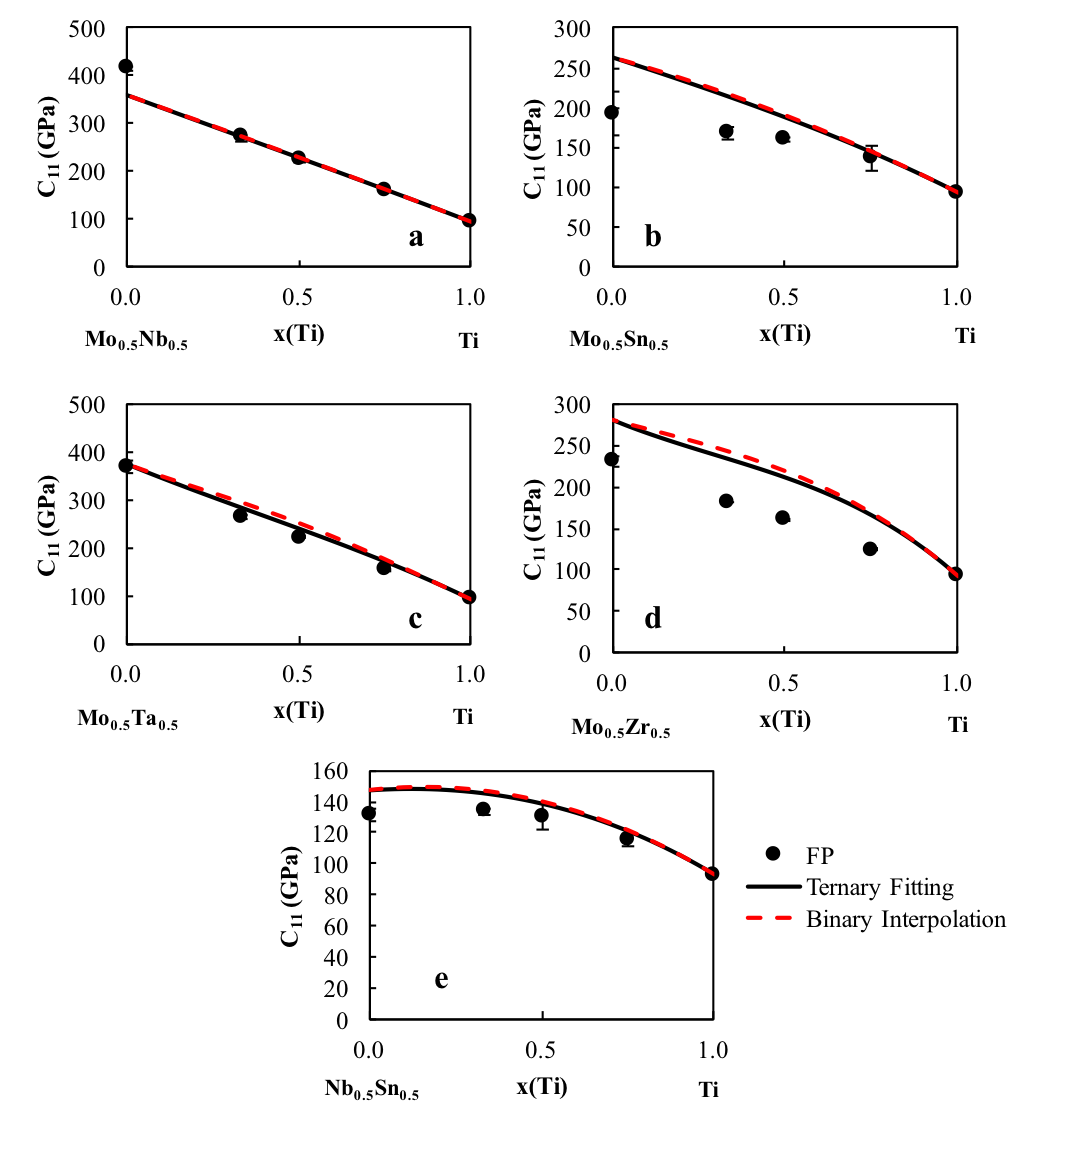
\includegraphics[width=\textwidth]{Chapter-6/Figures/tixyc111.png}
	\caption{$\overline{C}_{11}$ values (circles) from the current first-principles calculations plotted with their errors as well as the current modeling with (black solid line) and without ternary interaction parameters (red dashed line) for five of the Ti-X-Y binary systems from a 50-50 mixture of the alloying elements X$_{0.5}$Y$_{0.5}$ to Ti (X $\neq$ Y = Mo, Nb, Ta, Sn, Zr).}
	\label{Ch6-figure:tixyc11_1}
\end{figure}

\pagebreak
\begin{figure}[H]
	\centering
	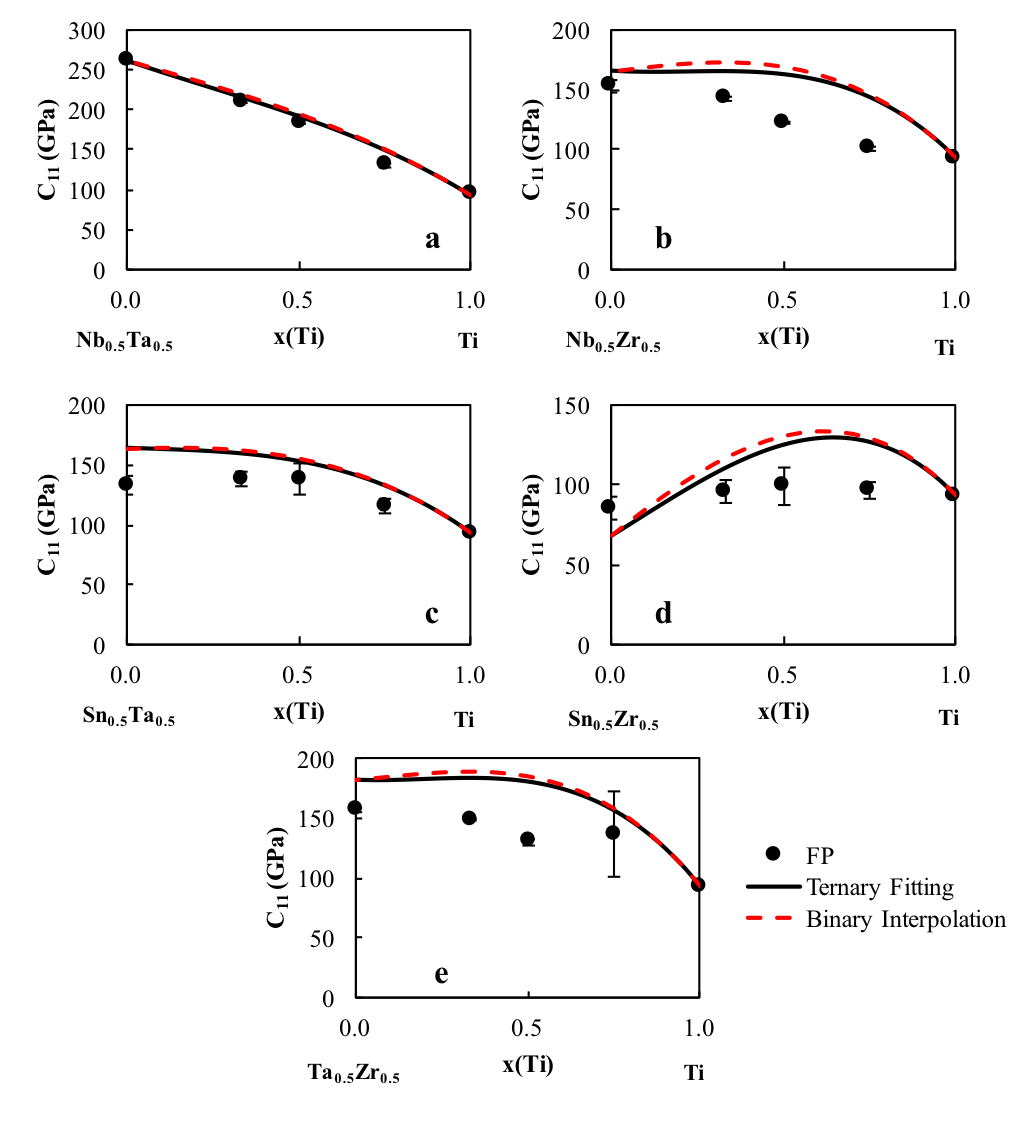
\includegraphics[width=\textwidth]{Chapter-6/Figures/tixyc112.png}
	\caption{$\overline{C}_{11}$ values (circles) from the current first-principles calculations plotted with their errors as well as the current modeling with (black solid line) and without ternary interaction parameters (red dashed line) for five of the Ti-X-Y binary systems from a 50-50 mixture of the alloying elements X$_{0.5}$Y$_{0.5}$ to Ti (X $\neq$ Y = Mo, Nb, Ta, Sn, Zr).}
	\label{Ch6-figure:tixyc11_2}
\end{figure}


\pagebreak
\begin{figure}[H]
	\centering
	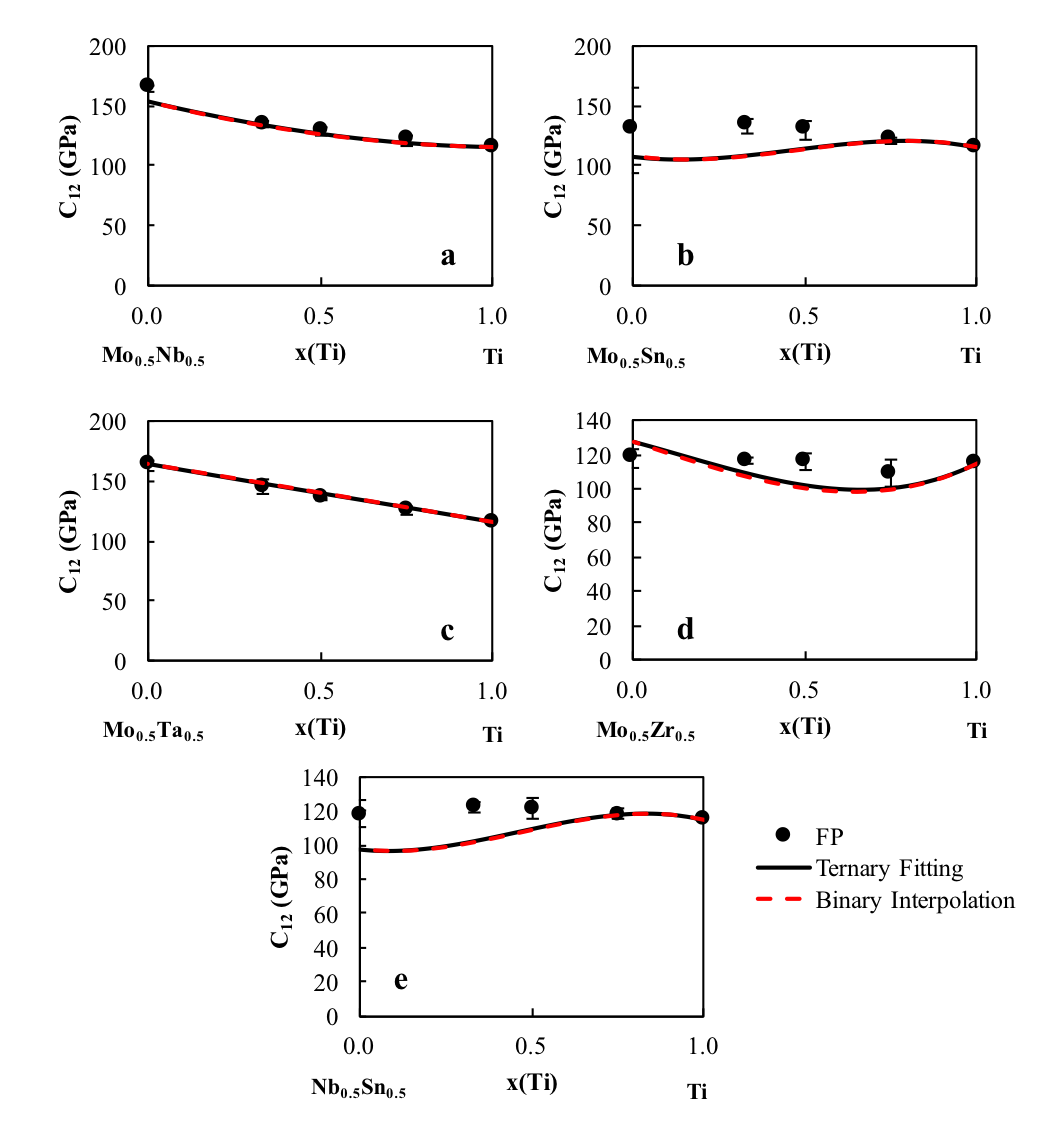
\includegraphics[width=\textwidth]{Chapter-6/Figures/tixyc121.png}
	\caption{$\overline{C}_{12}$ values (circles) from the current first-principles calculations plotted with their errors as well as the current modeling with (black solid line) and without ternary interaction parameters (red dashed line) for five of the Ti-X-Y binary systems from a 50-50 mixture of the alloying elements X$_{0.5}$Y$_{0.5}$ to Ti (X $\neq$ Y = Mo, Nb, Ta, Sn, Zr).}
	\label{Ch6-figure:tixyc12_1}
\end{figure}

\pagebreak
\begin{figure}[H]
	\centering
	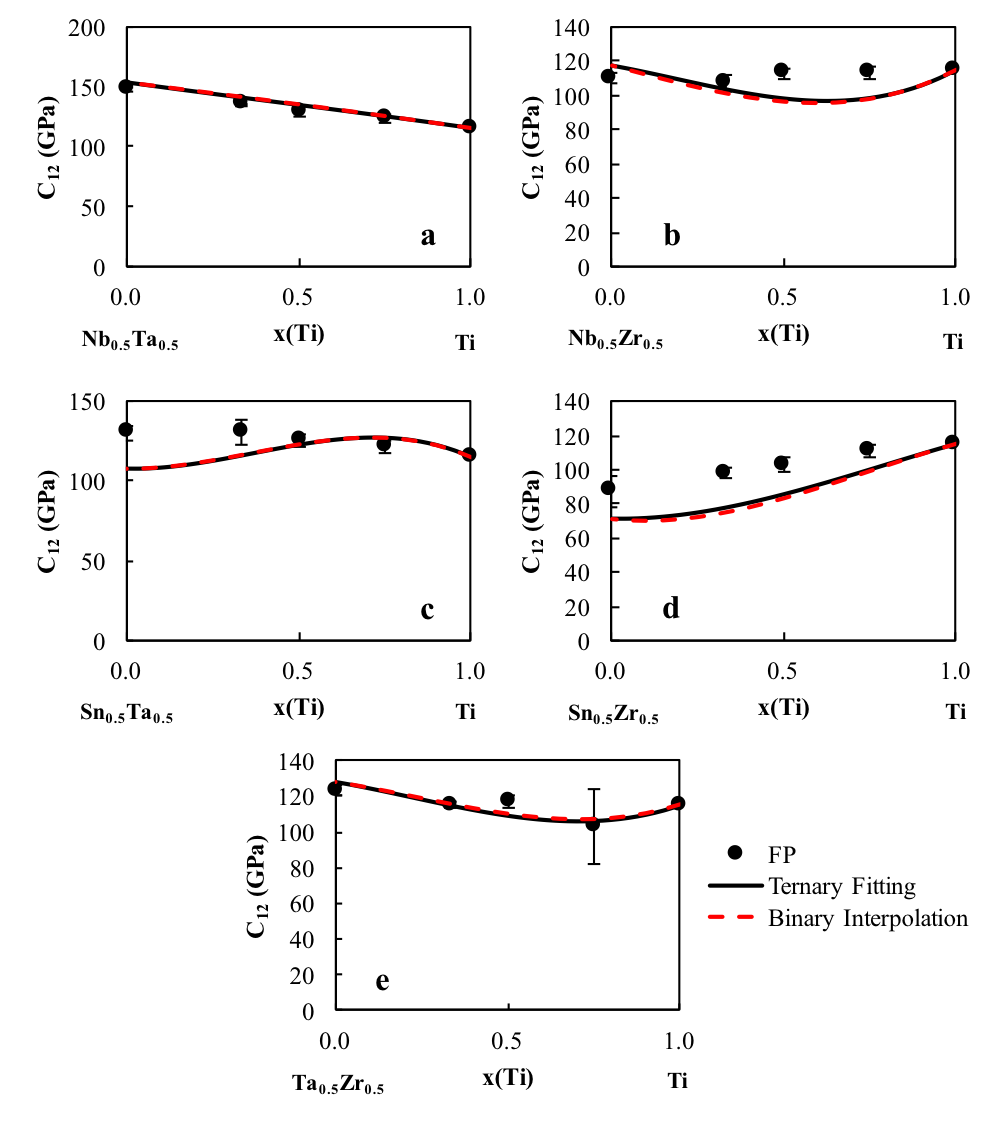
\includegraphics[width=\textwidth]{Chapter-6/Figures/tixyc122.png}
	\caption{$\overline{C}_{12}$ values (circles) from the current first-principles calculations plotted with their errors as well as the current modeling with (black solid line) and without ternary interaction parameters (red dashed line) for five of the Ti-X-Y binary systems from a 50-50 mixture of the alloying elements X$_{0.5}$Y$_{0.5}$ to Ti (X $\neq$ Y = Mo, Nb, Ta, Sn, Zr).}
	\label{Ch6-figure:tixyc12_2}
\end{figure}

\pagebreak
\begin{figure}[H]
	\centering
	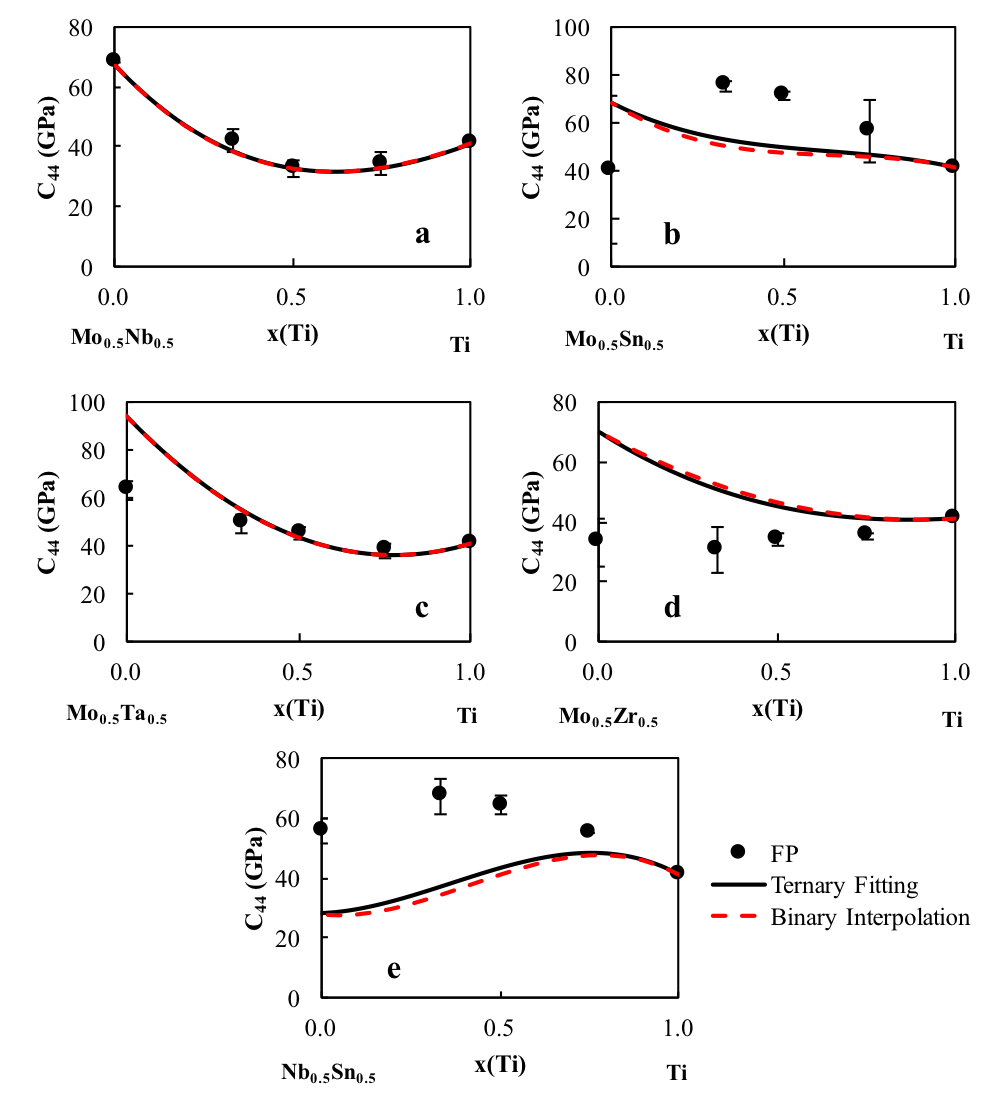
\includegraphics[width=\textwidth]{Chapter-6/Figures/tixyc441.png}
	\caption{$\overline{C}_{44}$ values (circles) from the current first-principles calculations plotted with their errors as well as the current modeling with (black solid line) and without ternary interaction parameters (red dashed line) for five of the Ti-X-Y binary systems from a 50-50 mixture of the alloying elements X$_{0.5}$Y$_{0.5}$ to Ti (X $\neq$ Y = Mo, Nb, Ta, Sn, Zr).}
	\label{Ch6-figure:tixyc44_1}
\end{figure}

\pagebreak
\begin{figure}[H]
	\centering
	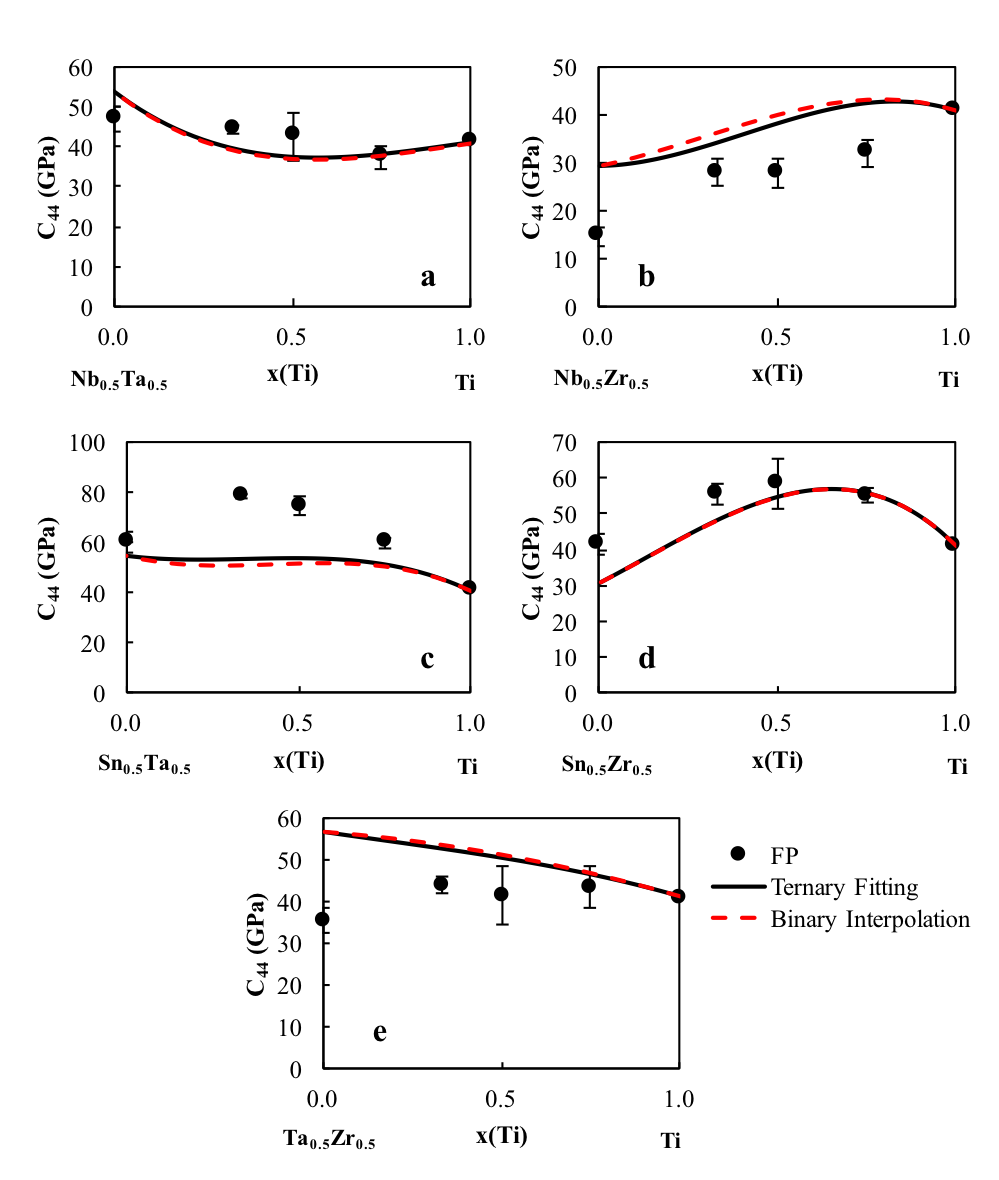
\includegraphics[width=\textwidth]{Chapter-6/Figures/tixyc442.png}
	\caption{$\overline{C}_{44}$ values (circles) from the current first-principles calculations plotted with their errors as well as the current modeling with (black solid line) and without ternary interaction parameters (red dashed line) for five of the Ti-X-Y binary systems from a 50-50 mixture of the alloying elements X$_{0.5}$Y$_{0.5}$ to Ti (X $\neq$ Y = Mo, Nb, Ta, Sn, Zr).}
	\label{Ch6-figure:tixyc44_2}
\end{figure}

\pagebreak
\begin{figure}[H]
	\centering
	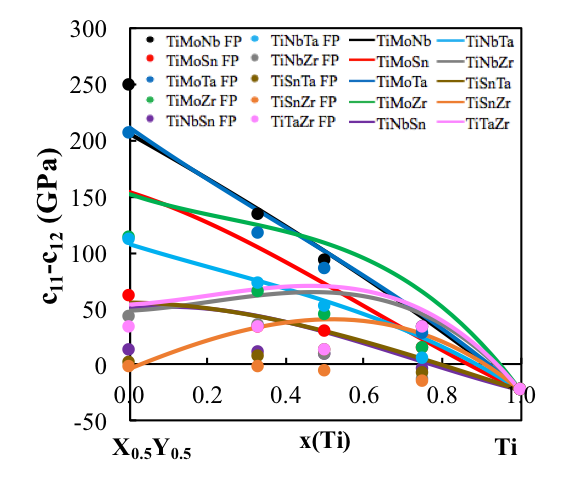
\includegraphics{Chapter-6/Figures/tixyc11-c12.png}
	\caption{$\overline{C}_{11}$-$\overline{C}_{12}$ values (symbols) from the current first-principles calculations plotted with the current modeling (lines) plotted from a 50-50 mixture of the alloying elements X and Y to Ti (X $\neq$ Y = Mo, Nb, Ta, Sn, Zr). The $\overline{C}_{11}$-$\overline{C}_{12}$ shows the stability of the bcc phase, when the value is negative the bcc phase is not stable in the corresponding composition ranges.}
	\label{Ch6-figure:tixyc11-c12}
\end{figure}

\pagebreak
\begin{figure}[H]
	\centering
	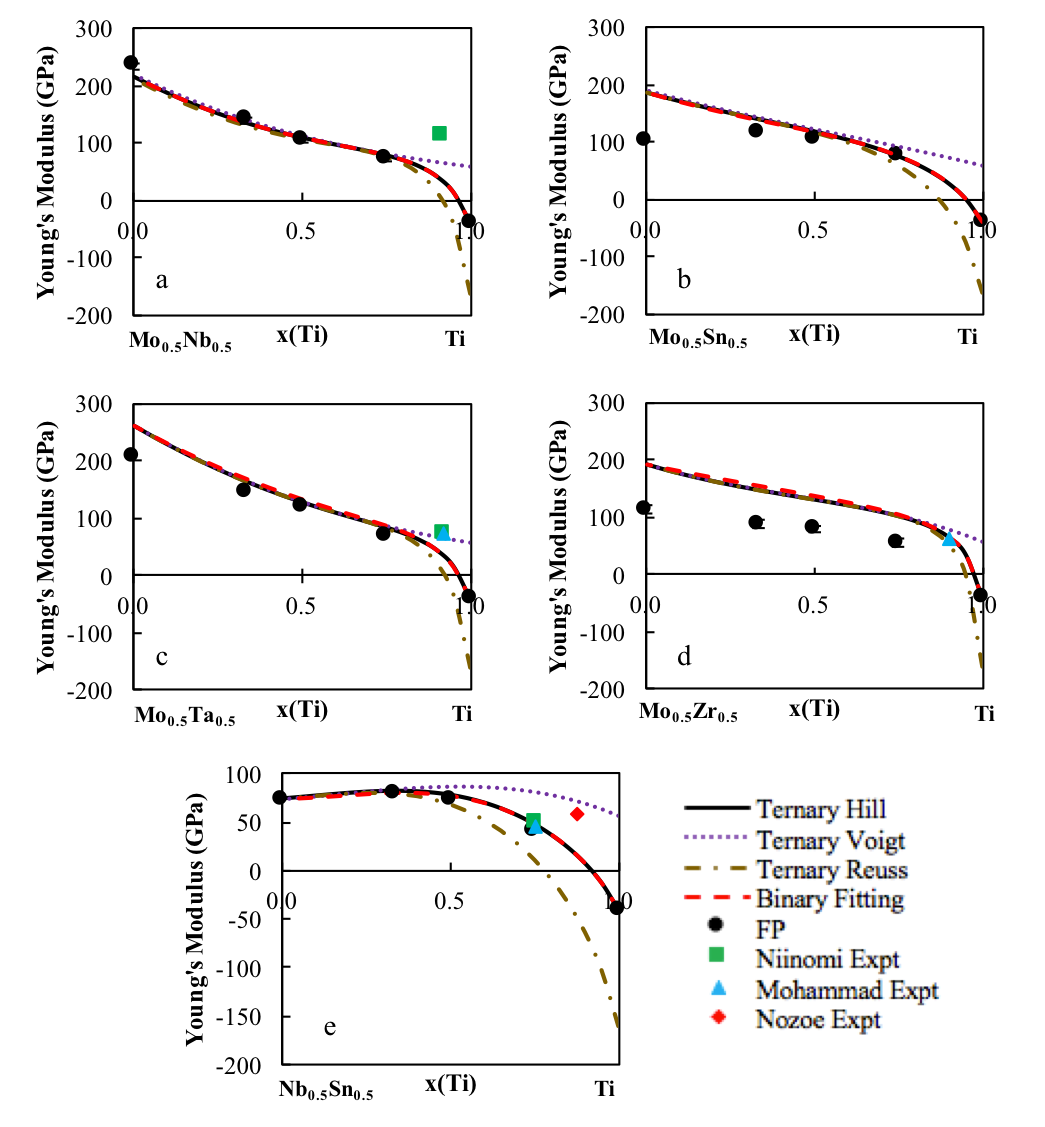
\includegraphics[width=\textwidth]{Chapter-6/Figures/tixyyoungs1.png}
	\caption{Young's modulus of five Ti-X-Y ternary systems plotted from a 50-50 mixture of the alloying elements to Ti in the bcc phase. The present calculations are plotted as filled circles with the error bars. The red dotted line is without the ternary interaction parameters. The dotted purple line is the Voigt upper Young's modulus bound, the gold dot dashed line is the lower Reuss Young's modulus bound and the black line is the Hill Young's modulus average. Experimental values are included for comparison \cite{Niinomi2012,Mohammed2014,Nozoe2007,Geetha2009}.}
	\label{Ch6-figure:tixyyoungs1}
\end{figure}

\pagebreak
\begin{figure}[H]
	\centering
	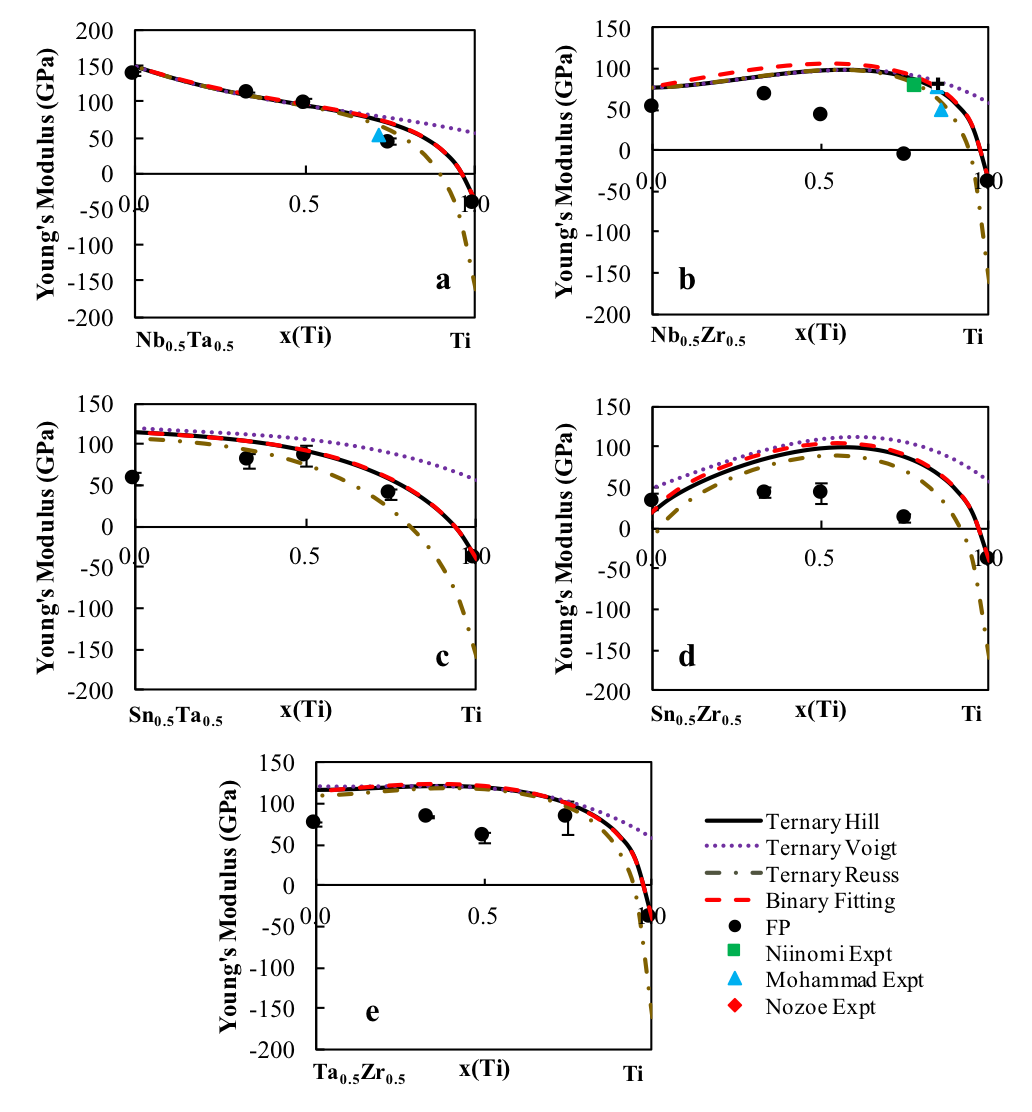
\includegraphics[width=\textwidth]{Chapter-6/Figures/tixyyoungs2.png}
	\caption{Young's modulus of five Ti-X-Y ternary systems plotted from a 50-50 mixture of the alloying elements to Ti in the bcc phase. The present calculations are plotted as filled circles with the error bars. The red dotted line is without the ternary interaction parameters. The dotted purple line is the Voigt upper Young's modulus bound, the gold dot dashed line is the lower Reuss Young's modulus bound and the black line is the Hill Young's modulus average. Experimental values are included for comparison \cite{Niinomi2012,Mohammed2014,Nozoe2007,Geetha2009}.}
	\label{Ch6-figure:tixyyoungs2}
\end{figure}

\pagebreak
\begin{figure}[H]
	\centering
	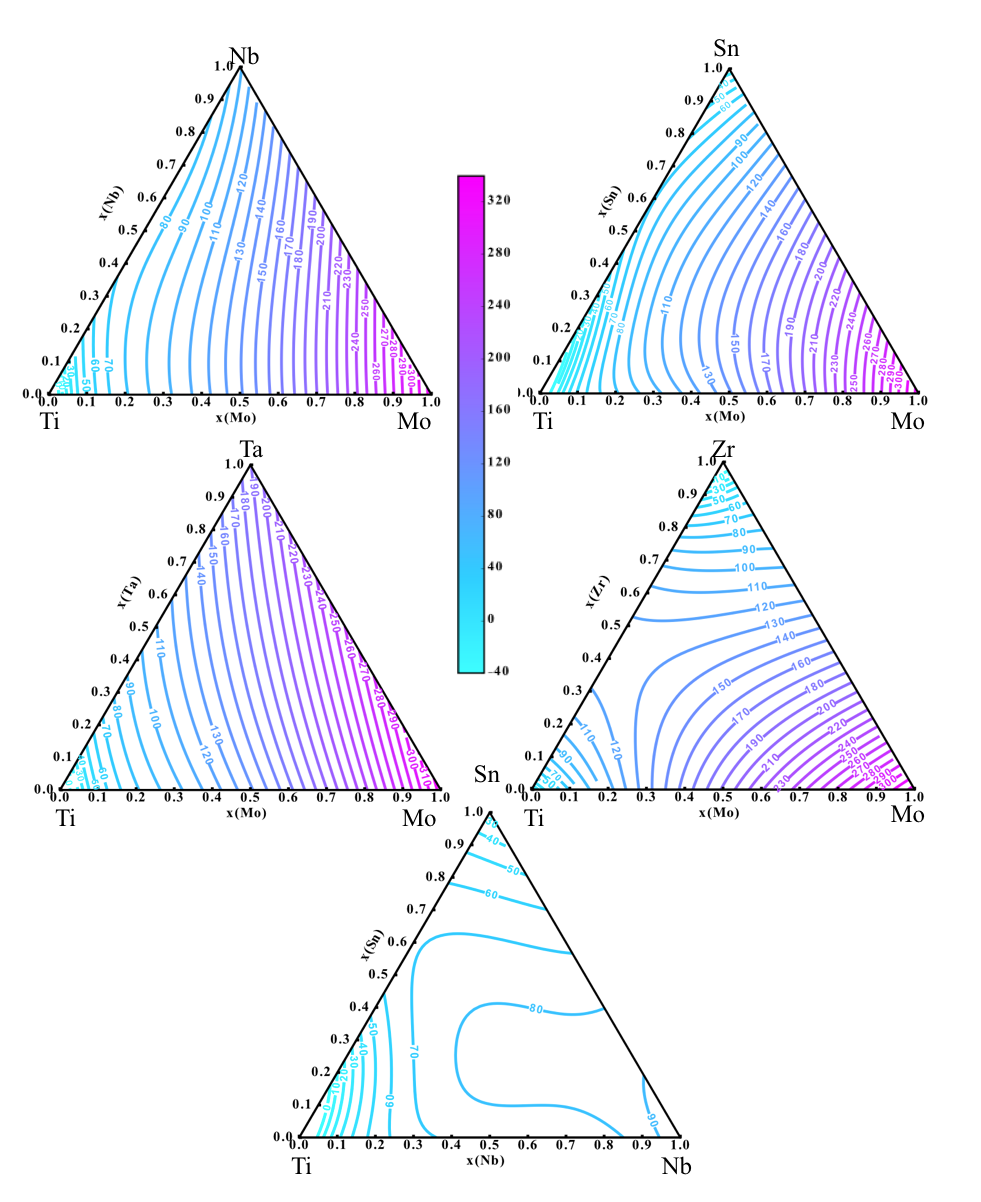
\includegraphics[width=\textwidth]{Chapter-6/Figures/tixymap1.png}
	\caption{Young's modulus in GPa mapped as a function of composition for the Ti-Mo-Nb, Ti-Mo-Sn, Ti-Mo-Ta, Ti-Mo-Zr and Ti-Nb-Sn alloy systems using pycalphad \cite{Otis2017}.}
	\label{Ch6-figure:tixymap1}
\end{figure}

\pagebreak
\begin{figure}[H]
	\centering
	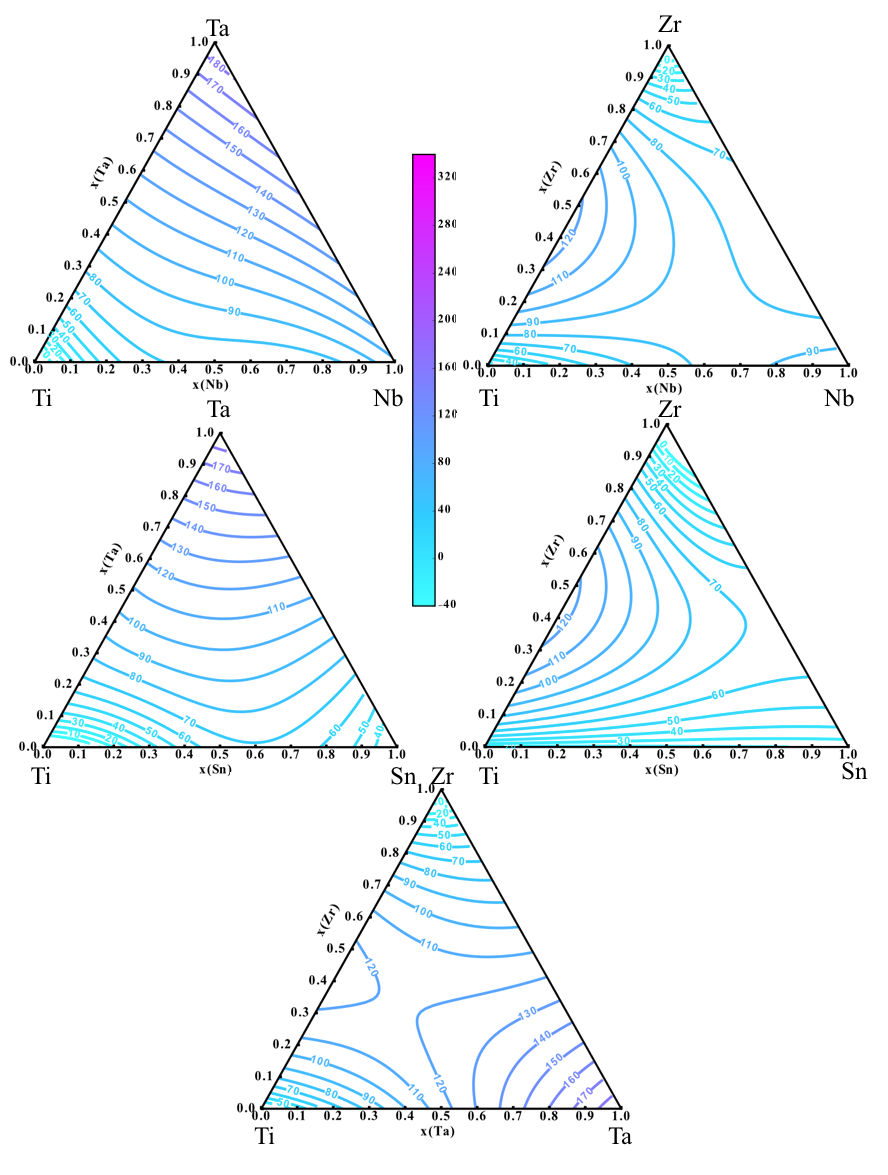
\includegraphics[width=\textwidth]{Chapter-6/Figures/tixymap2.png}
	\caption{Young's modulus in GPa mapped as a function of composition for the Ti-Mo-Nb, Ti-Mo-Sn, Ti-Mo-Ta, Ti-Mo-Zr and Ti-Nb-Sn alloy systems using pycalphad \cite{Otis2017}.}
	\label{Ch6-figure:tixymap2}
\end{figure}

\pagebreak
\begin{figure}[H]
	\centering
	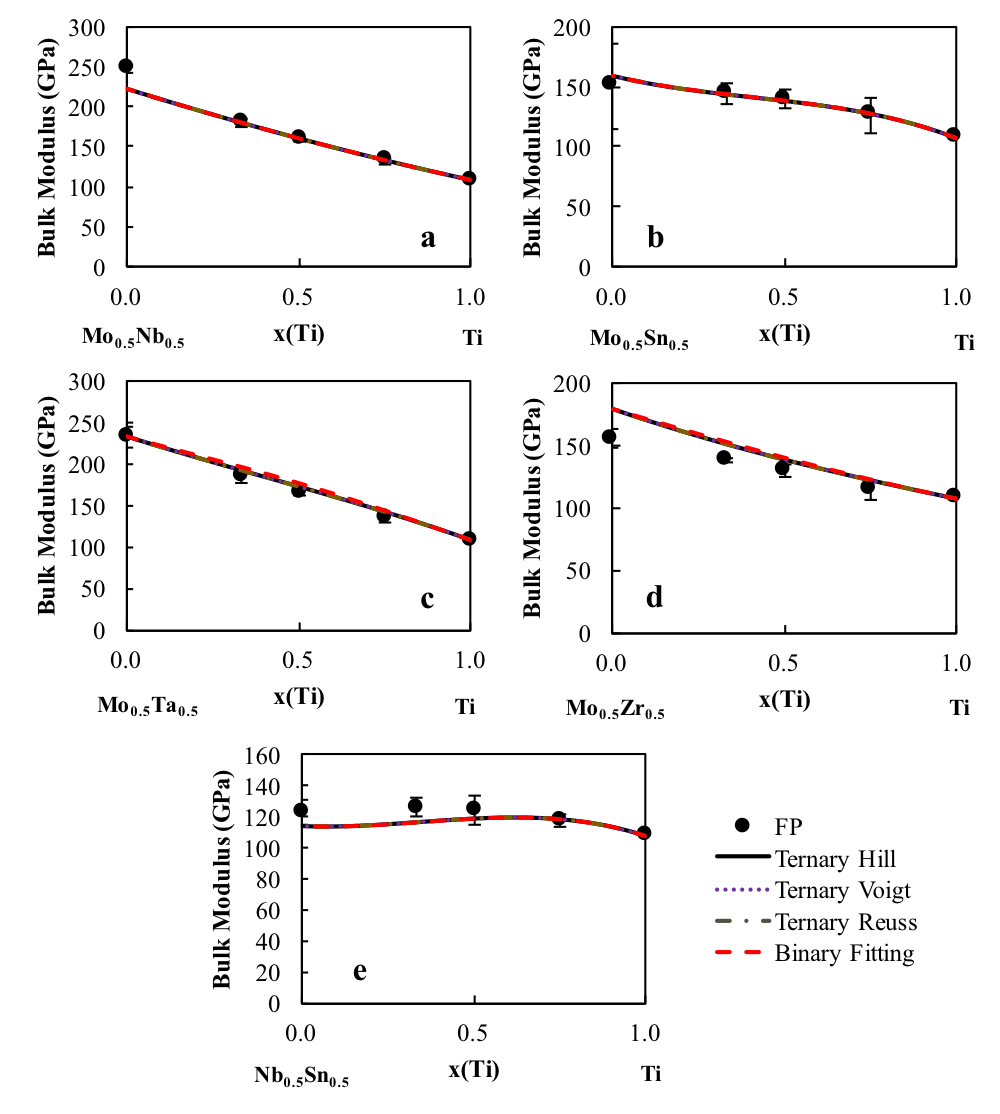
\includegraphics[width=\textwidth]{Chapter-6/Figures/tixybulk1.png}
	\caption{Bulk modulus in GPa mapped as a function of composition for the Ti-Mo-Nb, Ti-Mo-Sn, Ti-Mo-Ta, Ti-Mo-Zr and Ti-Nb-Sn alloy systems using pycalphad \cite{Otis2017}.}
	\label{Ch6-figure:tixybulk1}
\end{figure}

\pagebreak
\begin{figure}[H]
	\centering
	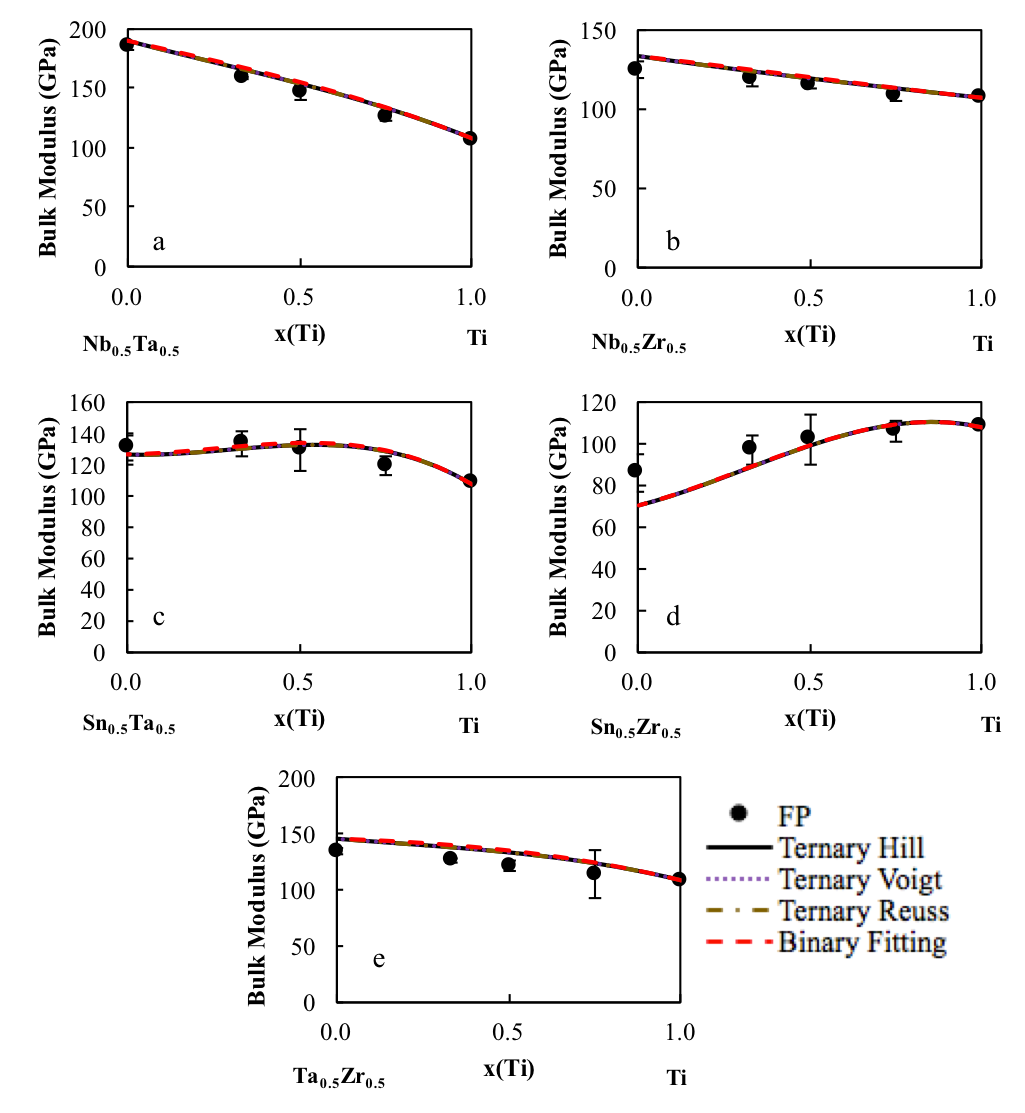
\includegraphics[width=\textwidth]{Chapter-6/Figures/tixybulk2.png}
	\caption{Bulk modulus in GPa mapped as a function of composition for the Ti-Nb-Ta, Ti-Nb-Zr, Ti-Sn-Ta, Ti-Sn-Zr and Ti-Ta-Zr alloy systems using pycalphad \cite{Otis2017}.}
	\label{Ch6-figure:tixybulk2}
\end{figure}

\pagebreak
\begin{figure}[H]
	\centering
	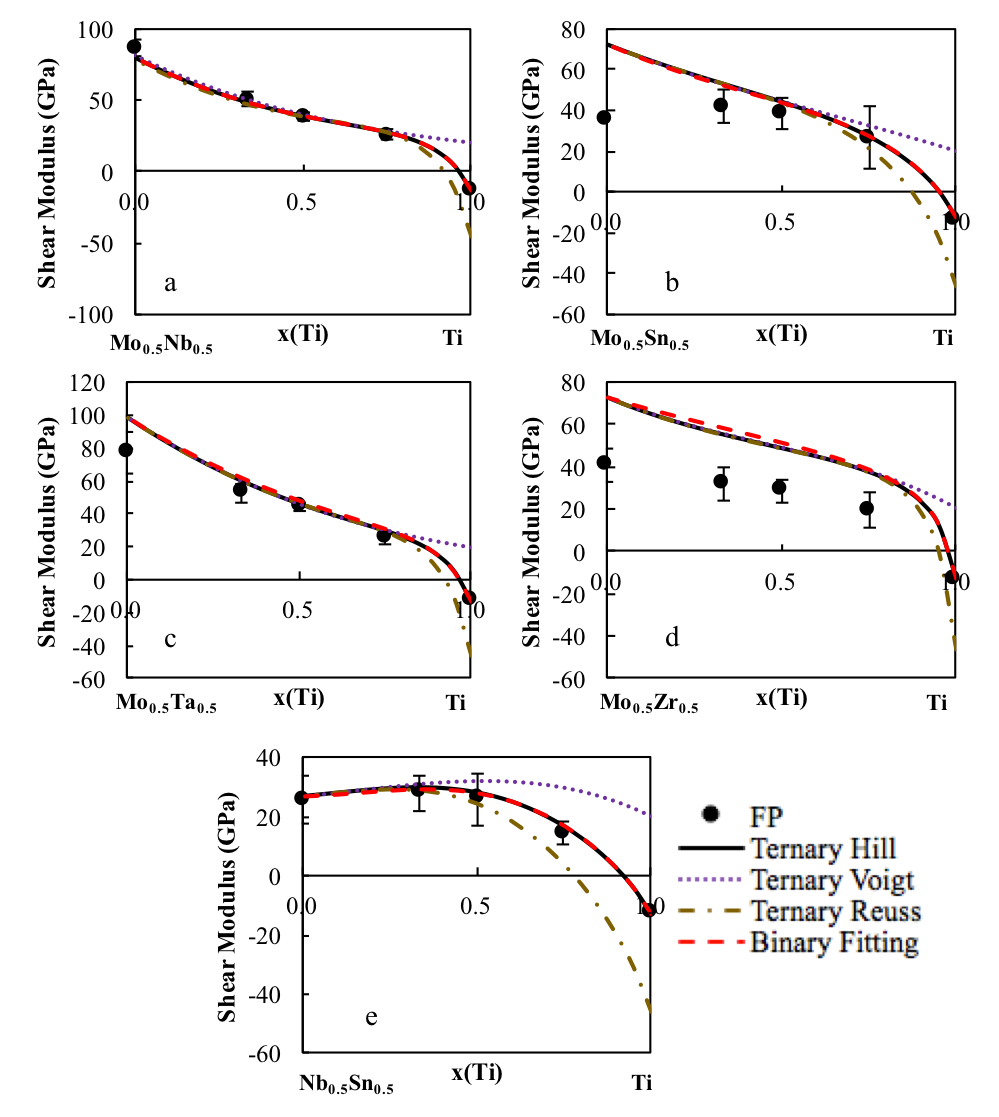
\includegraphics[width=\textwidth]{Chapter-6/Figures/tixyshear1.png}
	\caption{Shear modulus in GPa mapped as a function of composition for the Ti-Mo-Nb, Ti-Mo-Sn, Ti-Mo-Ta, Ti-Mo-Zr and Ti-Nb-Sn alloy systems using pycalphad \cite{Otis2017}.}
	\label{Ch6-figure:tixyshear1}
\end{figure}

\pagebreak
\begin{figure}[H]
	\centering
	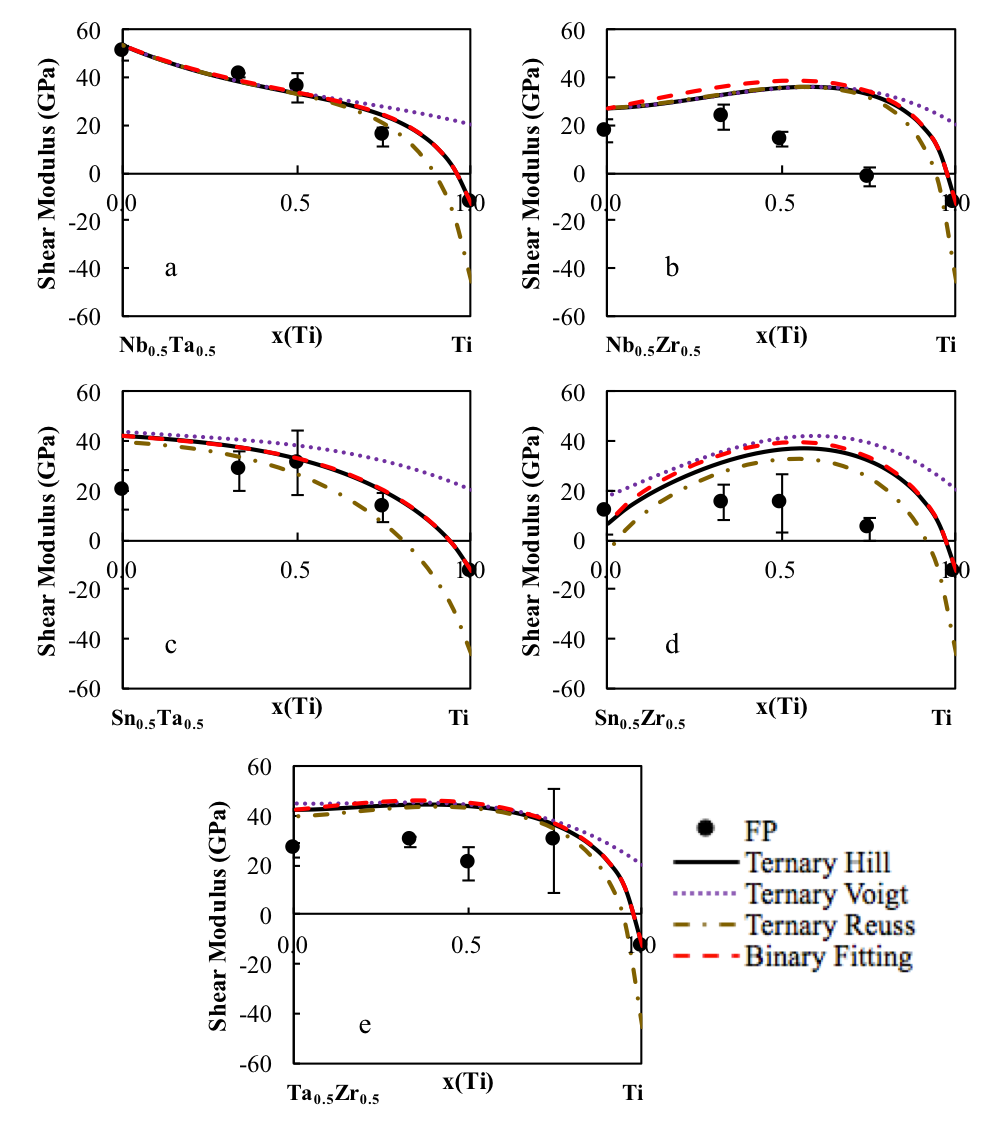
\includegraphics[width=\textwidth]{Chapter-6/Figures/tixyshear2.png}
	\caption{Shear modulus in GPa mapped as a function of composition for the Ti-Nb-Ta, Ti-Nb-Zr, Ti-Sn-Ta, Ti-Sn-Zr and Ti-Ta-Zr alloy systems using pycalphad \cite{Otis2017}.}
	\label{Ch6-figure:tixyshear2}
\end{figure}

\pagebreak
\begin{figure}[H]
	\centering
	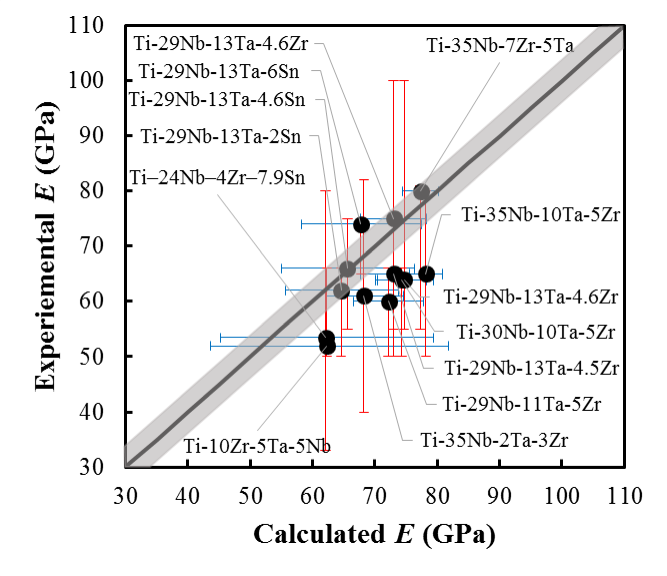
\includegraphics{Chapter-6/Figures/tixydatabase.png}
	\caption{$E$ of multicomponent bcc Ti alloys predicted from the database compared with measured experimental results. Vertical error bars plotted are from the variation in experimental data for given multi-component alloys, and horizontal error bars Voigt-Reuss bounds from the DFT-based first-principles. The grey region refers to the error introduced from the elastic stiffness coefficients in the first-principles calculations. More information on the alloys is Table \ref{Ch6-table:tixydatacomp} \cite{Mohammed2014,Geetha2009,Tane2010a}.}
	\label{Ch6-figure:tixydatabase}
\end{figure}